\documentclass[conference]{IEEEtran}
\IEEEoverridecommandlockouts
% The preceding line is only needed to identify funding in the first footnote. If that is unneeded, please comment it out.
\usepackage{cite,url}
\usepackage{amsmath,amssymb,amsfonts}
\usepackage{algorithmic}
\usepackage{graphicx}
\usepackage{textcomp}
\usepackage{soul,xcolor}
\usepackage{easyReview}

\usepackage{booktabs,array} % Packages for tables
\usepackage[inline]{enumitem}

\usepackage[format=default,justification=centerlast]{caption} % Figure caption text customization

\usepackage[list=true,labelformat=simple]{subcaption}
\renewcommand\thesubfigure{(\alph{subfigure})}


\usepackage{tikz}
\usetikzlibrary{shapes,arrows, positioning, quotes}
\usetikzlibrary{arrows.meta, positioning, decorations.markings}
\usetikzlibrary{calc,tikzmark}
\usetikzlibrary{backgrounds,calc,patterns,decorations.pathmorphing,decorations.markings,shapes,arrows,snakes,tikzmark}
\usepackage{siunitx}

\graphicspath{%
  {figs/matlab/}
}
\def\BibTeX{{\rm B\kern-.05em{\sc i\kern-.025em b}\kern-.08em
    T\kern-.1667em\lower.7ex\hbox{E}\kern-.125emX}}
\begin{document}

\title{Data-Driven Hardware-in-the-Loop Plant Modeling for Self-Driving Vehicles\\
\thanks{This work was partially supported by AutonomouStuff (https://autonomoustuff.com/)}
}


\author{\IEEEauthorblockN{Hannah Grady, Nicholas Nauman, and Md Suruz Miah}
\IEEEauthorblockA{\textit{Department of Electrical and Computer Engineering} \\
\textit{Bradley University}\\
Peoria, Illinois, 61615, USA \\
E-mail: \{hgrady,nnauman\}@mail.bradley.edu, smiah@bradley.edu }
}

\maketitle

\begin{abstract}

  In this paper, we present data-driven hardware-in-the-loop (HIL) plant models of different subsystems of a self-driving vehicle. Despite numerous concerns, the automotive industry is still investing remarkable resources into the production of self-driving vehicles. Among the challenges in the development process of such vehicles are the validation and testing process of various subsystems. Here we provide data-driven models of different subsystems so that the  automotive industry can validate and test autonomous vehicles without the need of a physical vehicle, which would reduce the considerable amount of cost to the automotive industry. The vehicle subsystems considered in this work include the steering, acceleration, brake, shift, speed, and speed control subsystems. Each of these subsystems is either a multi-input single output or single-input single output system. A Lexus RX450H self-driving vehicle is employed to collect raw data (inputs and outputs data for different subsystems) offline. We used the deep learning toolbox available in the commercial software package, MATLAB/SIMULINK, for modeling each of these systems. The contribution of this paper is twofold. First, collecting real time raw data from a physical Lexus RX450H vehicle and using it to develop machine learning models to represent the vehicle subsystems. Second, subsystem models created using machine learning tools for the Lexus vehicle are tested using Hardware-in-the-Loop. Therefore, the results of such modeling could be used for validation and testing without the need for a physical self-driving vehicle. The proposed modeling results could be useful for reducing the cost of the vehicle development process, since a physical vehicle is not required for validation and testing. 
  
  %However, the performance of the steering, acceleration, and brake subsystems demonstrated for conciseness purpose. .

\end{abstract}

\begin{IEEEkeywords}
Data-driven modeling, deep learning, hardware-in-the-loop, self-driving vehicle, vehicle subsystems
\end{IEEEkeywords}

\section{Introduction}
\label{sec:introduction}

%\todo[inline]{NN/HG: Add 2/3 sentences on what motivated the company to model
%  subsystems of autonomous vehicles, Hint: Erik mentioned already that employees
%can perform testing without the physical vehicle. You just need to extend his statement to write the motivational paragraph behind this project}

Due to the escalating demand for self-driving vehicles, the automotive industry is gradually shifting its attention toward manufacturing a variety of autonomous vehicles. The advancement of new technologies has led the automotive industry to develop such vehicles for commercial and personal use, with the aim to reduce crashes, energy consumption, pollution and congestion. However, the development process for autonomous vehicles still faces significant challenges. Each self-driving vehicle is composed of various subsystems that researchers of the autonomous vehicle community analyze, design, develop, and test.  Intuitively, self-driving vehicles require thorough testing at the factory level before they can be used by the public. Such a testing procedure for each physical vehicle is inefficient and costly, as it involves the testing of different vehicle subsystems, such as the steering, brake and shift subsystems. In this work, we model different modules/subsystems of a self-driving vehicle using machine learning techniques, where a physical self-driving vehicle is not required for testing.



Note that modeling vehicle subsystems is a pre-requisite for the development of reliable controllers for autonomous vehicles to be managed in the era of modern transportation systems. In particular, this work models different subsystems for a self-driving vehicle of the vehicle fleet shown in Fig.~\ref{fig:fleet}. %
%
\begin{figure}[htbp]
  \centering
  \includegraphics[scale=0.15]{figs/img/autonomousVehiclesAStuff}
  \caption{Autonomous vehicle fleet (courtesy of AutonomouStuff Inc., https://autonomoustuff.com)}
  \label{fig:fleet}
\end{figure}
%
%Such modeling process would allow companies to continue crucial deliveries or transports of their products even if there is a shortage of drivers. %
%
% \begin{figure}[htbp]
%   \centering
%   \begin{subfigure}[b]{0.48\linewidth}
%     \centering
%        \caption{}
%     \label{fig:fleet}
%   \end{subfigure}
%   \begin{subfigure}[b]{0.48\linewidth}
%     \centering
%
%     \caption{}
%     \label{fig:steerOverview}
%   \end{subfigure}
%   \caption{\subref{fig:fleet} Autonomous vehicle fleet in AutonomouStuff Solutions and \subref{fig:steerOverview} steering model setup (courtesy of AutonomouStuff). }
%   \label{fig:AstuffFleetSteeringSetup}
% \end{figure}


Autonomous vehicles have the ability to make roads safer for drivers
and pedestrians alike. To develop a reliable and safe transportation system for the 
modern world, a large body of research in the field of autonomous vehicles has
been generated~\cite{Liu2017,Prasad2020}. In fact, the research on this topic has been conducted from a variety of perspectives, such as the application of connected and autonomous vehicle technology~\cite{DoT2017}, and the navigation and path control of self-driving vehicles~\cite{Duong2018,Chajan2021}. Authors in~\cite{Saruchi2015} worked on active front steering for a steer-by-wire vehicle. The steering system of high speed intelligent vehicles has been modeled using system identification~\cite{Li1999}. Therefore, it is clear that a large amount of research pertaining to self-driving vehicles has been pursued, especially in the past two decades. There are two operating modes considered for the autonomous vehicle employed in this work: %
%
\begin{itemize}
  \item Manual-drive and
  \item by-wire or autonomous~\cite{Saruchi2015}.
\end{itemize}
%
Manual-drive operation occurs when the driver has complete control over the vehicle; including controlling the steering, speed, acceleration and braking of the vehicle. Autonomous operation occurs when the vehicle is controlled by a computer under driver supervision.
%
Usually, there are six main subsystems of a self-driving vehicle: %
%
\begin{enumerate*}
\item  Steering,

\item acceleration,

\item brake,

\item shift,

\item speed, and

\item speed control (cruise).
\end{enumerate*}
%
These subsystems are modeled in order to get an accurate representation of how
the vehicle is to be controlled. %
%Within the scope of this project and to expedite the modeling process, commercially available modeling tools in Mathworks' MATLAB, System Identification app in the System Identification Toolbox and Neural Network Time Series app in the Deep Learning toolbox, were used to model six subsystems for a Lexus vehicle platform, which is an experimental autonomous vehicle platform that belongs to AutonomouStuff Solutions~\footnote{\url{https://autonomoustuff.com/}}. By creating these software models, the company can run tests using them without needing the physical vehicle. As a result, these models could potentially allow the company to get more testing done.
%
The first subsystem we shall model is the steering model, and then we will move onto
the other subsystems. There are already controllers in place for the Lexus
vehicle platform, but their ability to match the desired input specified by the vehicle operator
%\comment{reliability}{Need to define what do you mean by reliability, be very specific}
is lower than expected due to the non-linear
behaviors of the torque voltages required to control each subsystem. The scope
of this project includes developing mathematical and/or data-driven models for each subsystem so that one can easily implement control systems that improve the reliability of the
autonomous vehicle platform. These models will be considered reliable if they can track actual vehicle subsystem behaviors with a minimum best fit percentage between 85 to 95 percent and fall within the error bounds defined for each subsystem. Once these models are developed, they will be tested using a Hardware-in-the-Loop (HIL) bench.
Once there is confidence in each model, these models can be used on the HIL bench to develop controllers that will remove the non-linear behaviors of each vehicle subsystem.


\section{Self-Driving Vehicle Subsystems}
\label{sec:selfDrivingVehicleOverview}

In this section, we illustrate subsystems of the self-driving vehicle; highlighting the hardware-in-the-loop modeling process conducted in the work. %
As mentioned, we focus on  six  main subsystems which are the steering, acceleration, brake, speed, shift, and speed control systems. Fig.~\ref{fig:highLevelSystemArchitecture} outlines these six subsystems in a Lexus vehicle similar to the one provided by the company, Hexagon $|$ AutonomouStuff (www.autonomoustuff.com). %
%
\begin{figure}[htbp]
  \centering
  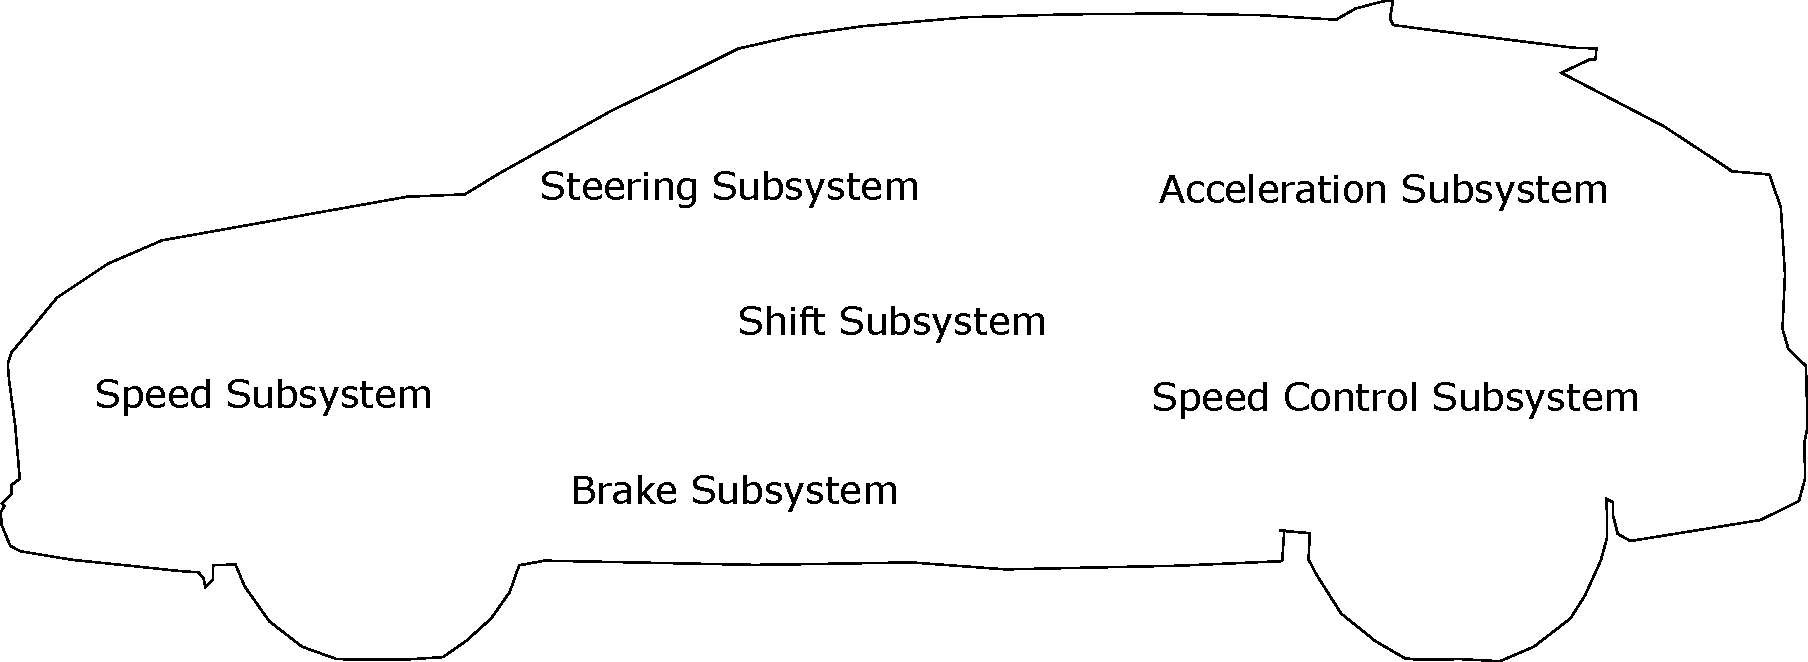
\includegraphics[height=3cm]{figs/inkscape/carSystemModelOutline}
  \caption{Hexagon Lexus self-driving vehicle showing different subsystems}
  \label{fig:highLevelSystemArchitecture}
\end{figure}
%
However, the actual self-driving vehicle (Lexus RX450H) that is used for collecting input-output data for all of these subsystems is shown in the picture of Fig.~\ref{fig:lexusvehicle}. A team of the project members visited the site to collect raw data for modeling the steering, brake, and acceleration subsystems of the vehicle. %
%
\begin{figure}[htbp]
	\centering
	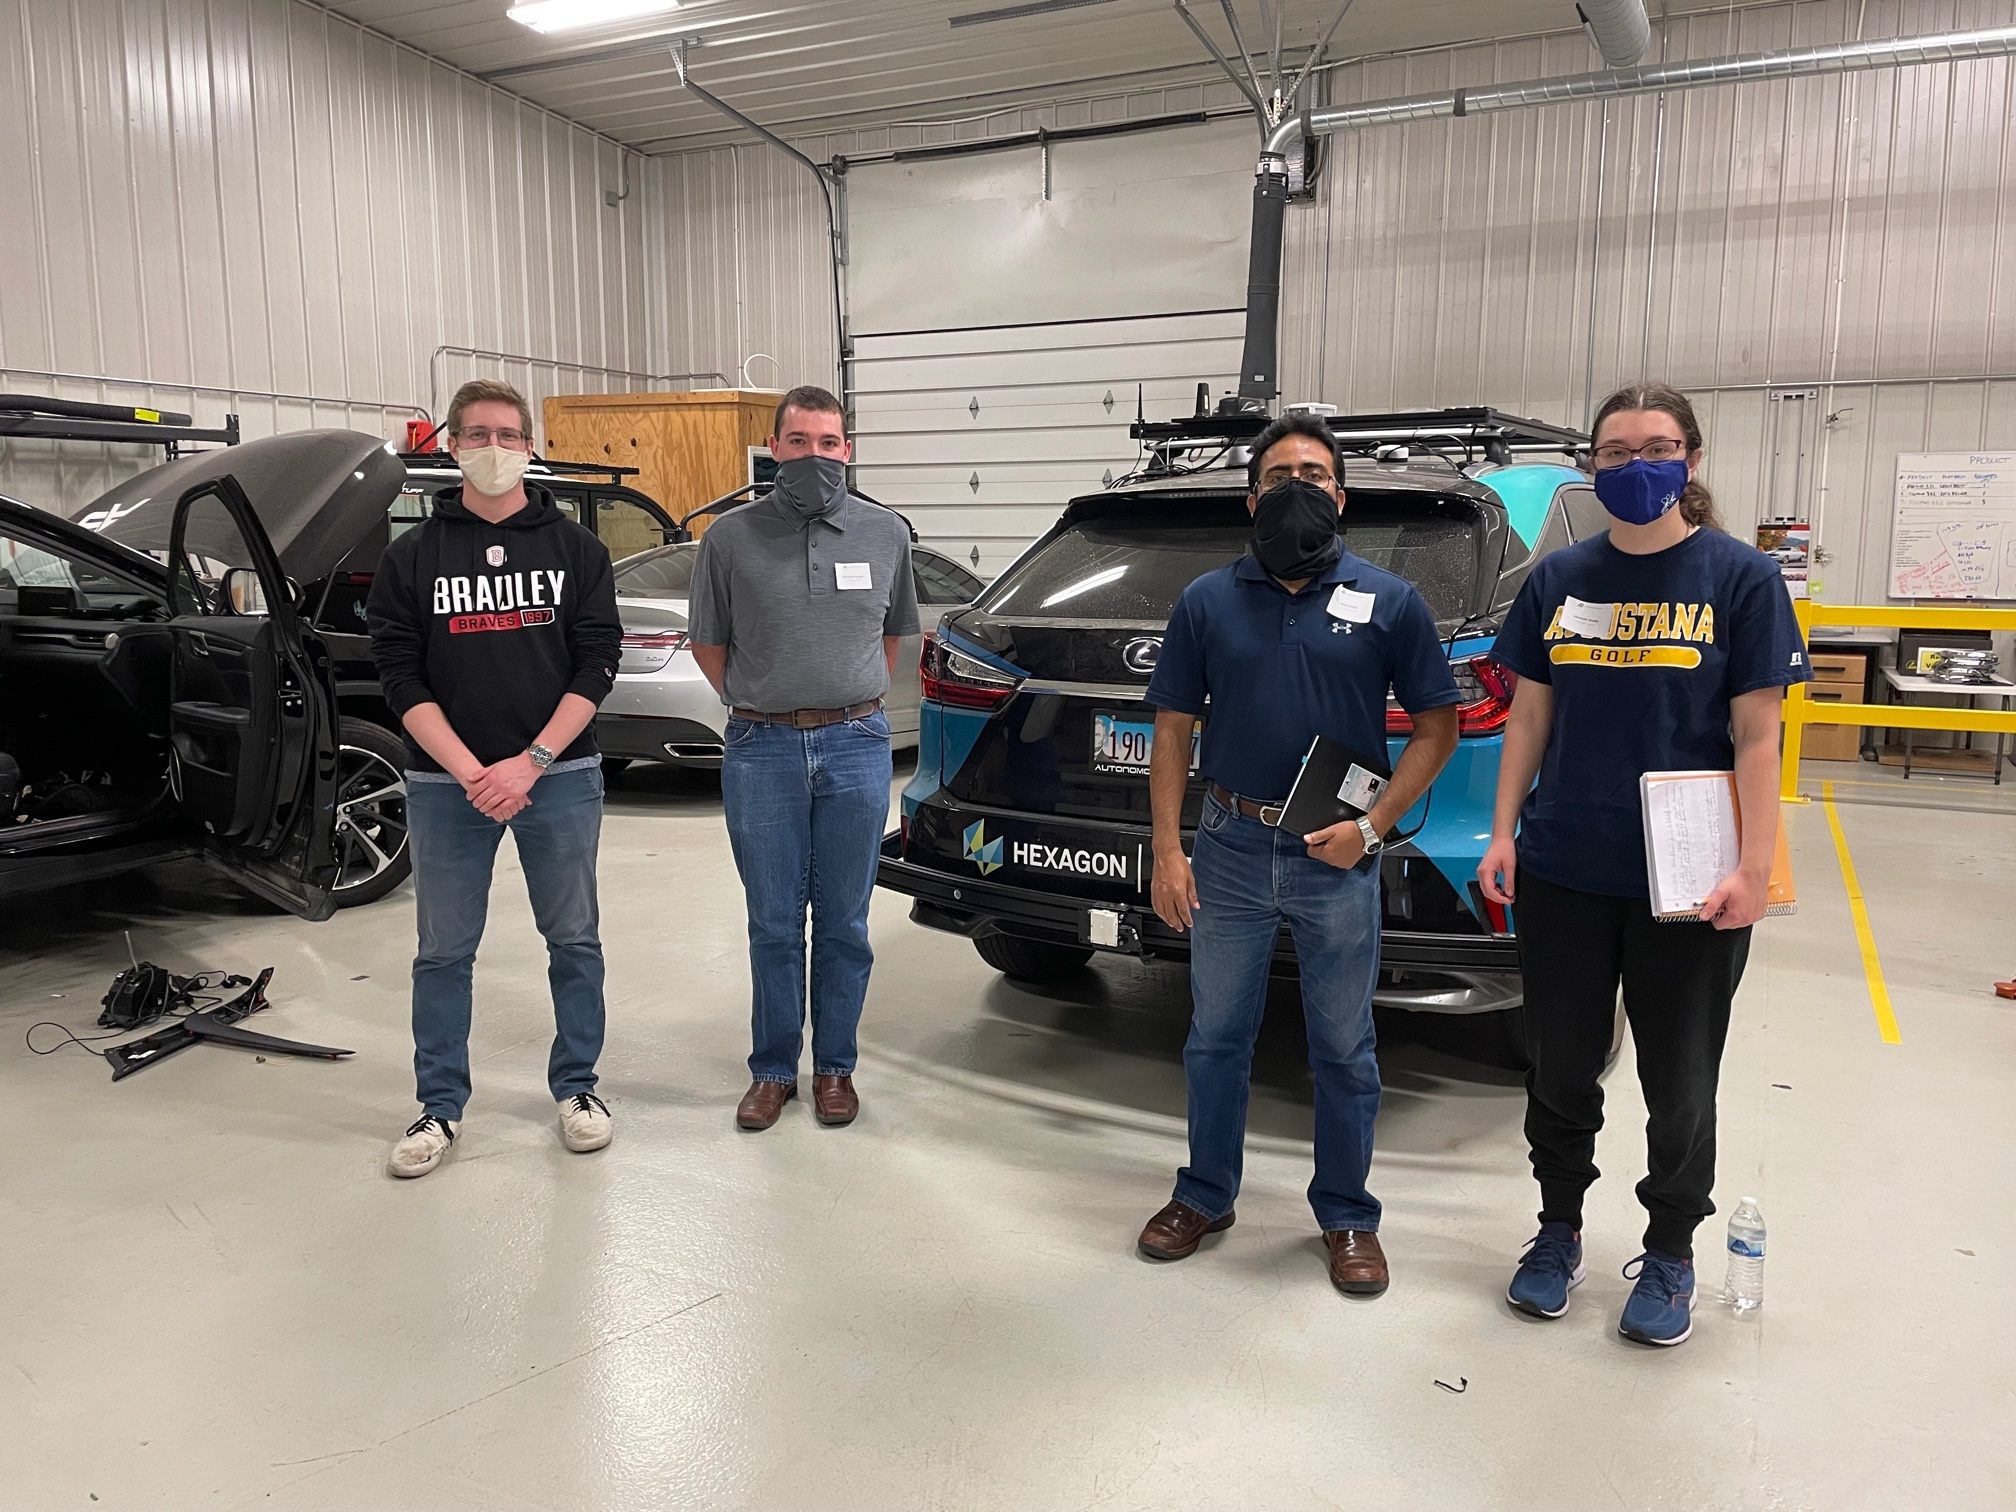
\includegraphics[height=4cm]{figs/img/picturesVisitToAStuff/visitors1-20211007}
	\caption{AutonomouStuff Lexus RX450H vehicle.}
	\label{fig:lexusvehicle}
\end{figure}
%


Each of the six subsystems will be treated as a multiple-input single-output (MISO) system. For each subsystem, every input that is a torque voltage is actually two torque voltage signals, and thus cannot be treated as a single input. The brake subsystem is shown to have two outputs, but the behaviors of one of the outputs is already known, so it will be modeled based on the other output's behavior. In the following sections we give a brief description of each of the subsystems of the self-driving vehicle modeled in this work. Each subsystem sends torque voltages to a motor that will control the subsystem.

\subsection{Steering Subsystem}
\label{sec:steeringSubsystem}

The steering subsystem of a generic self-driving vehicle consists of the steering arm, knuckle, rods, drag link, steering gear box, drop arm, cross shaft, steering column, steering shaft, and steering wheel~\footnote{\url{https://www.theengineerspost.com/car-steering-system-in-automobile/}}. Fig.~\ref{fig:steerOverview} depicts steering subsystems in the by-wire (autonomous) mode.  %
%
\begin{figure}[htbp]
  \centering
  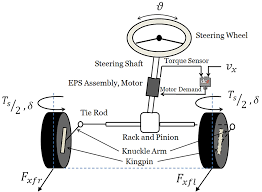
\includegraphics[scale=0.8]{figs/img/autonomousVehiclesSteering}
  \caption{Steering subsystem in autonomous mode (courtesy of Autonomoustuff.com).}
  \label{fig:steerOverview}
\end{figure}
%
In Fig.~\ref{fig:steerOverview}, the motor would
turn the pinion arms which would change the steering angle of the vehicle. The idea of by-wire mode for other vehicle subsystems is controlled in a similar manner with torque voltages being applied to a motor that controls the vehicle subsystem.


The ultimate goal of this subsystem is to control the steering angle for the vehicle to navigate in the desired heading. Therefore, the control system is designed to produce appropriate voltages to be applied to the power steering motors for the steering orient in the target direction. The block diagram of the control system designed for this subsystem is shown in Fig.~\ref{fig:steeringModelBlockDiagram}, where the target and the actual orientations of the vehicle are denoted by $\theta^{\text{ref}}$ and $\theta(t)$ at time $t\ge 0,$ respectively. %
%
\begin{figure}[htbp]
  \centering
  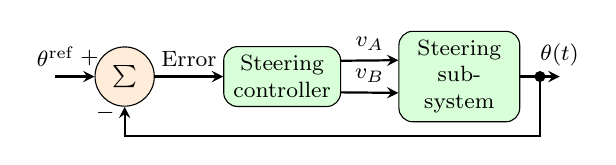
\begin{tikzpicture}
    \tikzstyle{every node} = [font=\footnotesize]
    \tikzstyle{block} = [draw, rectangle, fill=green!15, rounded corners=5pt, minimum width=1 cm, minimum height=0.75 cm]
    \tikzstyle{sum} = [draw, circle,fill=orange!15]
    % place nodes
    \node[sum](sum){$\sum$};
    \node[block,right of=sum,node distance=2 cm, text width=1.25cm,text centered](steeringController){Steering controller};
    \node[block,right of=steeringController,node distance=2.25 cm, text width=1.3cm,text centered](steeringSubsystem){Steering subsystem};

    % Connections
    \draw[stealth-,thick]
    (sum.west)--node[very near start,above]{$+$}++(-0.5,0)node[above]{$\theta^{\text{ref}}$};
    \draw[-stealth,thick]
    (sum.east)--node[midway,above]{Error}(steeringController);
    \draw[-stealth,thick]
    (steeringController.15)--node[midway,above]{$v_A$}(steeringSubsystem.165);
    \draw[-stealth,thick]
    (steeringController.-15)--node[midway,above]{$v_B$}(steeringSubsystem.-165);
    \draw[-stealth,thick]
    (steeringSubsystem.east) --coordinate (tt) ++(0.5,0)node[above]{$\theta(t)$};
    \fill
    (tt) circle [radius=2pt];
    \draw[-stealth,thick]
    (tt) -- ++(0,-0.75) -|(sum.south)node[pos=0.9,left]{$-$};
  \end{tikzpicture}
  % \captionsetup{justification=centering, margin=3cm}
  % 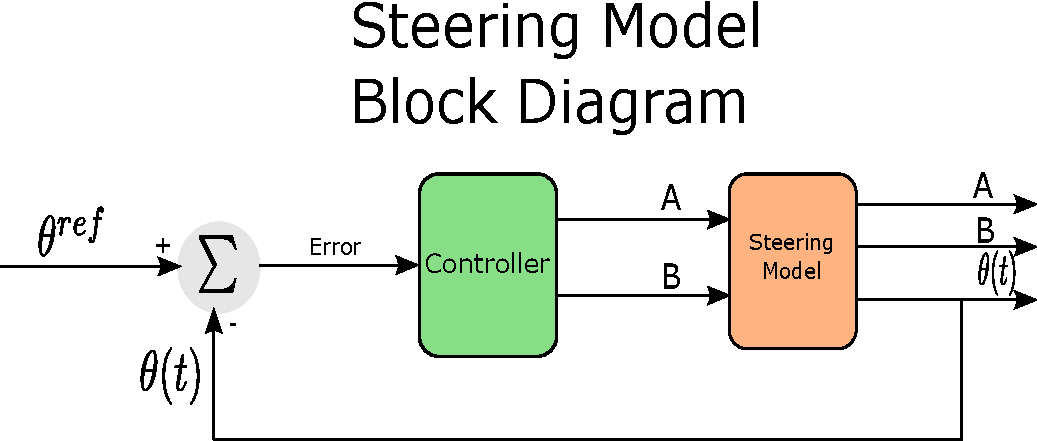
\includegraphics[width=2.5in]{figs/inkscape/steeringModelBlockDiagram}
  \caption{Steering subsystem block diagram.}
  \label{fig:steeringModelBlockDiagram}
\end{figure}
%
The torque voltages applied to the power steering motor are denoted by $v_{A}$ and $v_{B},$ respectively. These voltages are taken from a torque sensor located on the vehicle's steering column. The error signal, which is the difference between the target and the actual steering angles of the vehicle, is passed on to the steering controller. The outputs of the steering controller are the torque voltages that are applied to the power steering motors of the steering subsystems of the vehicle.


  \subsection{Brake Subsystem}
  The brake subsystem is made up of the master cylinder, brake rotor, brake drum, brake pad, brake caliper, brake shoe, brake booster, brake pedal, wheel speed sensors, ABS module, and brake lines~\footnote{\url{https://oards.com/car-brake-system-components/}}. A high-level block diagrams showing the inputs and outputs of a conventional brake subsystem of a self-driving vehicle is shown in Fig.~\ref{fig:brakeModelArchitecture}. %
%
 \begin{figure}[htbp]
    \centering
  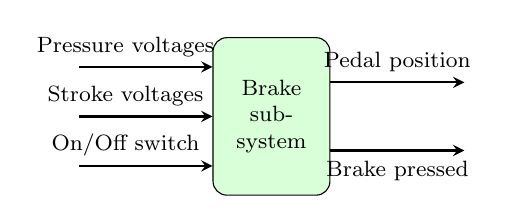
\begin{tikzpicture}
    \tikzstyle{every node} = [font=\footnotesize]
    \tikzstyle{block} = [draw, rectangle, fill=green!15, rounded corners=5pt, minimum width=1 cm, minimum height=2.0 cm]
    % place nodes
    \node[block,text width=1.25cm,text centered](brakeSubsystem){Brake subsystem};

    % Connections
    \draw[stealth-,thick]
    (brakeSubsystem.140)--node[pos=0.65,above]{Pressure voltages}++(-1.7,0);
    \draw[stealth-,thick]
    (brakeSubsystem.180)--node[pos=0.65,above]{Stroke voltages}++(-1.7,0);
    \draw[stealth-,thick]
    (brakeSubsystem.-140)--node[pos=0.65,above]{On/Off switch}++(-1.7,0);
    \draw[-stealth,thick]
    (brakeSubsystem.30)--node[pos=0.5,above]{Pedal position}++(1.7,0);
    \draw[-stealth,thick]
    (brakeSubsystem.-30)--node[pos=0.5,below]{Brake pressed}++(1.7,0);
  \end{tikzpicture}
    % \captionsetup{justification=centering, margin=3cm}
    % \includegraphics[width=2.5in]{figs/inkscape/brakeModelArchitecture}
    \caption{Brake subsystem block diagram}
    \label{fig:brakeModelArchitecture}
\end{figure}
%
The subsystem takes the brake pedal pressure voltages, brake pedal stroke voltages, and the brake pedal on/off switch values as inputs. Using these values, it generates a new brake pedal position (as a percentage) and a boolean value called brake pressed. This boolean value indicates to the user whether or not the brake pedal is being pressed.

\subsection{Acceleration Subsystem}

  The acceleration subsystem consists of the throttle pedal, engine, and crankshaft~\footnote{\url{https://harrisautomotiverepair.com/car-accelerator/}}. It is a multiple-input multiple-output system, whose block diagram is depicted in Fig.~\ref{fig:accelModelArchitecture}.
Taking the acceleration pedal voltages as the input, the subsystem then produces the acceleration pedal position as the output. The output represents how much the pedal is pressed as a percentage. %
%of the acceleration subsystem. %
%
 \begin{figure}[htbp]
    \centering
  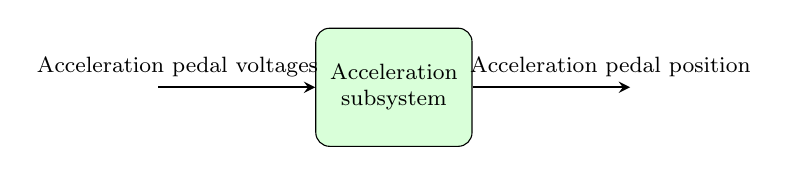
\begin{tikzpicture}
    \tikzstyle{every node} = [font=\footnotesize]
    \tikzstyle{block} = [draw, rectangle, fill=green!15, rounded corners=5pt, minimum width=1.5 cm, minimum height=1.5 cm]
    % place nodes
    \node[block,text width=1.75cm,text centered](accelSubsystem){Acceleration subsystem};
    % Connections
    \draw[stealth-,thick]
    (accelSubsystem.180)--node[very near end,above]{Acceleration pedal voltages}++(-2.0,0);
    \draw[-stealth,thick]
    (accelSubsystem.0)--node[very near end,above]{Acceleration pedal position}++(2.0,0);
  \end{tikzpicture}
    \caption{Acceleration subsystem block diagram}
    \label{fig:accelModelArchitecture}
 \end{figure}
% %
%\todo[inline]{Please see how I described block diagrams for steering, and brake subsystems. Use the same format for explaining all the subsystems.  You cannot just place a figure without referring and explaining the figure in the text.}
  \subsection{Shift Subsystem}
  The components that make up the shift subsystem are the friction clutch, bands, spring loaded valve, load sensor, shift valve, torque converter, gear stick, seals, and gasket~\footnote{\url{https://oards.com/car-automatic-transmission-system-components/}}. This subsystem can be classified as a single-input single-output system. %
%
  % A block diagram of the shift subsystem is seen in Fig.~\ref{fig:shiftModelArchitecture}.
  The subsystem takes the desired shifter gear value from the user as the input. Within the subsystem, the actual shifter gear is changed to better reflect the desired gear. This actual shifter gear value is then the output of the subsystem.
 % \begin{figure}[htbp]
 %    \centering
 %  \begin{tikzpicture}
 %    \tikzstyle{every node} = [font=\footnotesize]
 %    \tikzstyle{block} = [draw, rectangle, fill=green!15, rounded corners=5pt, minimum width=1.5 cm, minimum height=1.5 cm]
 %    % place nodes
 %    \node[block,text width=1.75cm,text centered](shiftSubsystem){Shift subsystem};

 %    % Connections
 %    \draw[stealth-,thick]
 %    (shiftSubsystem.180)--node[very near end,above]{Desired Shifter Gear}++(-1.9,0);
 %    \draw[-stealth,thick]
 %    (shiftSubsystem.0)--node[very near end,above]{Actual Shifter Gear}++(1.9,0);

 %  \end{tikzpicture}
 %    \caption{Shift subsystem block diagram}
 %    \label{fig:shiftModelArchitecture}
 % \end{figure}

 %
% \todo[inline]{Please see how I described block diagrams for steering, and brake subsystems. Use the same format for explaining all the subsystems.  You cannot just place a figure without referring and explaining the figure in the text.}
  \subsection{Speed Subsystem}
  The speed subsystem would fall under the multiple-input single-output system category. %A block diagram representation can be found in Fig.~\ref{fig:speedModelArchitecture}. %
  The subsystem has four inputs, the acceleration pedal position, brake pedal position, and shifter gear. Using these inputs, the speed subsystem finds the vehicle speed. This vehicle speed is then the output of the system.

%  \begin{figure}[htbp]
%     \centering
%   \begin{tikzpicture}
%     \tikzstyle{every node} = [font=\footnotesize]
%     \tikzstyle{block} = [draw, rectangle, fill=green!15, rounded corners=5pt, minimum width=1 cm, minimum height=2 cm]
%     % place nodes
%     \node[block,text width=1.25cm,text centered](speedSubsystem){Speed subsystem};

%     % Connections
%     \draw[stealth-,thick]
%     (speedSubsystem.140)--node[very near end,above]{Acceleration pedal position}++(-1.9,0);
%     \draw[stealth-,thick]
%     (speedSubsystem.180)--node[very near end,above]{Brake pedal position}++(-1.9,0);
%     \draw[stealth-,thick]
%     (speedSubsystem.-140)--node[near end,above]{Shifter Gear}++(-1.9,0);
%     \draw[-stealth,thick]
%     (speedSubsystem.0)--node[near end,above]{Vehicle Speed}++(1.9,0);

%   \end{tikzpicture}
%     % \captionsetup{justification=centering, margin=3cm}
%     % \includegraphics[width=2.5in]{figs/inkscape/brakeModelArchitecture}
%     \caption{Speed subsystem block diagram}
%     \label{fig:speedModelArchitecture}
% \end{figure}
% %
%\todo[inline]{Please see how I described block diagrams for steering, and brake subsystems. Use the same format for explaining all the subsystems.  You cannot just place a figure without referring and explaining the figure in the text.}

  \subsection{Speed Control Subsystem}
  The speed control subsystem components include the cruise control switch, vehicle speed sensor, throttle sensor, and brake switch~\footnote{\url{https://www.freeasestudyguides.com/electrical-cruise-control-systems.html}}. %This subsystem is a straightforward single-input single-output system, shown in Fig.~\ref{fig:speedControlModelArchitecture}. %
  The Desired Vehicle Speed input is set by the user and sent to the speed control subsystem. Taking this input, the subsystem updates the Actual Vehicle Speed to better reflect the desired value. This value is then sent out to the rest of the vehicle system.
 % \begin{figure}[htbp]
 %    \centering
 %  \begin{tikzpicture}
 %    \tikzstyle{every node} = [font=\footnotesize]
 %    \tikzstyle{block} = [draw, rectangle, fill=green!15, rounded corners=5pt, minimum width=1.5 cm, minimum height=1.5 cm]
 %    % place nodes
 %    \node[block,text width=1.75cm,text centered](speedControlSubsystem){Speed Control subsystem};

 %    % Connections
 %    \draw[stealth-,thick]
 %    (speedControlSubsystem.180)--node[very near end,above]{Desired Vehicle Speed}++(-1.9,0);
 %    \draw[-stealth,thick]
 %    (speedControlSubsystem.0)--node[very near end,above]{Actual Vehicle Speed}++(1.9,0);

 %  \end{tikzpicture}
 %    \caption{Speed Control subsystem block diagram}
 %    \label{fig:speedControlModelArchitecture}
 % \end{figure}
 %
% % \todo[inline]{Please see how I described block diagrams for steering, and brake subsystems. Use the same format for explaining all the subsystems.  You cannot just place a figure without referring and explaining the figure in the text.}

\section{Modeling Vehicle Subsystems}

To start the modeling process, we first collected raw data of the subsystems illustrated in the previous section. The input-output data were then used to model different subsystems of the self-driving vehicle using the deep learning toolbox available in the commercial modeling software SIMULINK\footnote{\url{https://www.mathworks.com/products/simulink.html}}. To demonstrate the modeling accuracy, to evaluate the effectiveness of our models, and to develop safe and reliable controllers for each subsystem, the following system requirements are to be met:


\begin{itemize}
  \item Each vehicle subsystem will be able to track nonlinearities %depicted in Fig.~\ref{fig:nonlinGraph} %
        associated with small changes in the output of each subsystem. %
  %
  % \begin{figure}[htbp]
  %   \centering
  %   \captionsetup{justification=centering}
  %   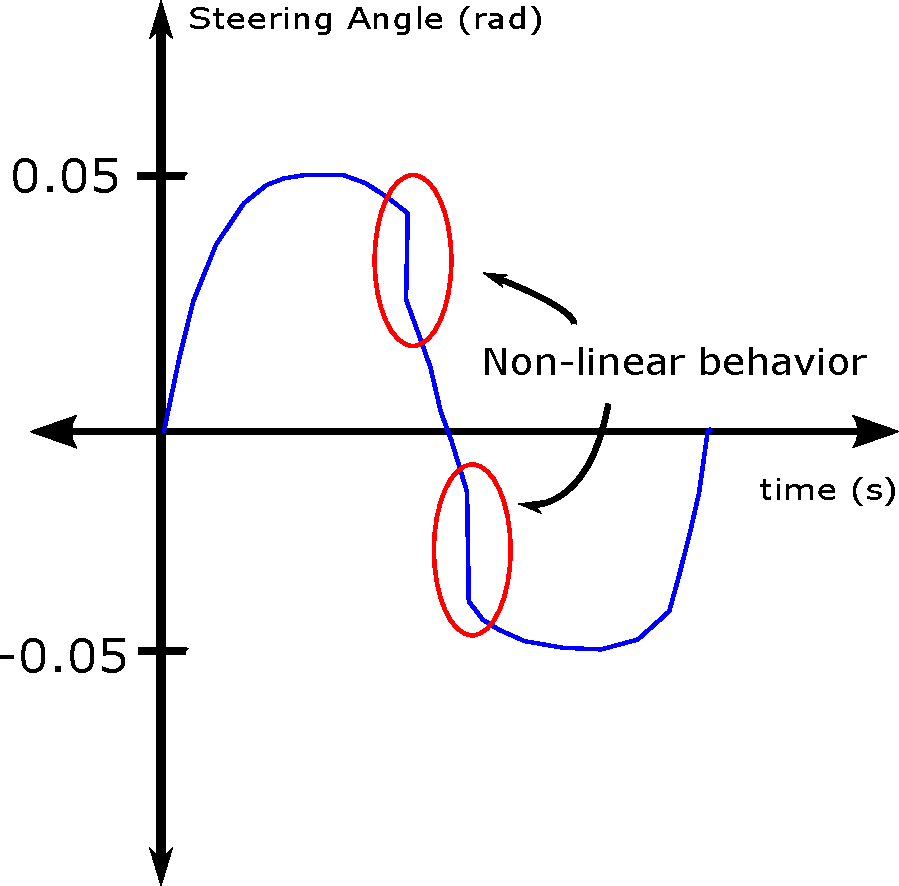
\includegraphics[width=2.5in]{figs/inkscape/nonlinearBehavior}
  %   \caption{Nonlinear behavior of steering subsystem.}
  %   \label{fig:nonlinGraph}
  % \end{figure}

\item Each vehicle subsystem plant model will track any desired inputs within the specified error bounds\add{:}
	\begin{itemize}
		\item Steering angle within 5 degrees
		\item Pedal positions within 5\%
	\end{itemize}
\item Each vehicle subsystem will be modeled independently from other vehicle subsystems
\end{itemize}
%
The vehicle plant models will satisfy the requirements listed below:
\begin{itemize}
    \item The resulting plant model will consist of accurate subsystem models, as defined above
    \item The subsystems can be used to create a hardware-in-the-loop (HIL) testbench
    \item The subsystems can handle very small changes in their output accurately
\end{itemize}
%

All of the subsystems have nonlinear behaviors when there are small changes in the output of the subsystem. The steering subsystem, for example, should behave in a smooth, continuous manner. However, a team of researchers from AutonomouStuff observed that when trying to implement features such as lane tracking for the Lexus vehicle platform,  the torque voltages would momentarily stall and then suddenly change when small changes in the steering angle (less than five degrees) occurred. This behavior %, depicted in Fig.~\ref{fig:nonlinGraph}, %
made it very challenging to complete features like lane tracking. The plant models developed in this work will aid in the development of controllers that will remove the nonlinearities, allowing features like lane tracking to be implemented in a safer, smoother manner.


\subsection{Steering System Modeling}
To develop a model of the steering system, we employed multiple methods. The first method that we tried was generating a NARX model and a transfer function model, making use of the System Identification Toolbox in MATLAB. The NARX model we developed was not accurate and did not track the output of the steering system data. The transfer function model we developed was more reliable tracking the output of the steering system data, but was unable to meet the error requirements, as there were sudden changes that forced high error peaks. Then we employed a neural network model, making use of the Neural Network Time Series Toolbox in MATLAB. With the neural network model, the model was able to reliably and accurately track the output of the steering system data and stayed within the error requirements.

\subsection{Acceleration System Modeling}
To develop a model of the acceleration system, we employed multiple methods. The first method that we tried was generating a NARX model and a transfer function model, making use of the System Identification Toolbox in MATLAB. The NARX model we developed was accurate for the by-wire model and tracked the output of the acceleration system data, but did not meet the error requirements. The transfer function model we developed was more reliable tracking the output of the acceleration system data for the manual mode operation, but was unable to meet the error requirements, due to sudden changes that caused high error peaks. We then tried using a neural network model, using the Neural Network Time Series Toolbox in MATLAB. The neural network model reliably and accurately tracked the output of the acceleration system data while staying within the error requirements.

\subsection{Brake System Modeling}
To create a brake system model, we first tried generating transfer function models using MATLAB’s System Identification Toolbox. After generating multiple transfer function models and trying many different data log combinations, we still couldn’t find a model that was completely accurate across all combinations and that was below the error bound of 5\% for all combinations. Once this became clear, neural network models were created using the Neural Network Time Series Toolbox provided by MATLAB to see if they could create accurate brake models. Using this we were able to create a model that accurately tracked the data we collected from the brake system and that stayed within the 5\% error bound.



\section{Validation and Testing} \label{sec:simresults}

\subsection{Experimental Setup}
\label{sec:experimentalSetup}

We visited the workplace of AutonomouStuff in order to collect
data from the steering, acceleration, and braking subsystems in an autonomous
vehicle. The data we collected will be used to generate and then verify our
models. We collected data on the Lexus RX450H vehicle platform shown in
Fig.~\ref{fig:lexusvehicle}. %
The following hardware components that were used to collect the data:
	\begin{itemize}
    		\item Laptop
    		\item PACMod ECU
    		\item CANCase
    		\item CAN bus
 	\end{itemize}
  %
The interfacing software, Vector CANAlyzer, installed in the laptop is used to pass commands or log data, such as steering angle or acceleration or brake pedal position. This data is sent or received using the CANCase and CAN bus. These are connected to the AutonomouStuff designed PACMod ECU, which sends torque voltages to the desired vehicle subsystem allowing the laptop to either control the desired vehicle system or log data. The Vector CANAlyzer software is installed on the laptop and is used to parse the collected data that is sent from the CANCase. This is how we were able to collect logs of data that we would use to develop plant models of the autonomous vehicle subsystems.


Each subsystem that we are modeling is set up in a similar manner. In manual mode, the torque voltages that control each subsystem are sent by the vehicle's electronic control unit (ECU). In order to control the vehicle autonomously, the vehicle subsystem switches to by-wire mode. In by-wire mode, the torque voltages from the vehicle's ECU are discarded by open-circuiting the motors that control each subsystem. Instead, the PACMod ECU built by AutonomouStuff sends the torque voltages to the motor using relays. In Fig.~\ref{fig:vehicleSetup}, the experimental setup for data collection is shown. %
%
\begin{figure}[htbp]
	\centering
  % \captionsetup{justification=centering, margin=3cm}
  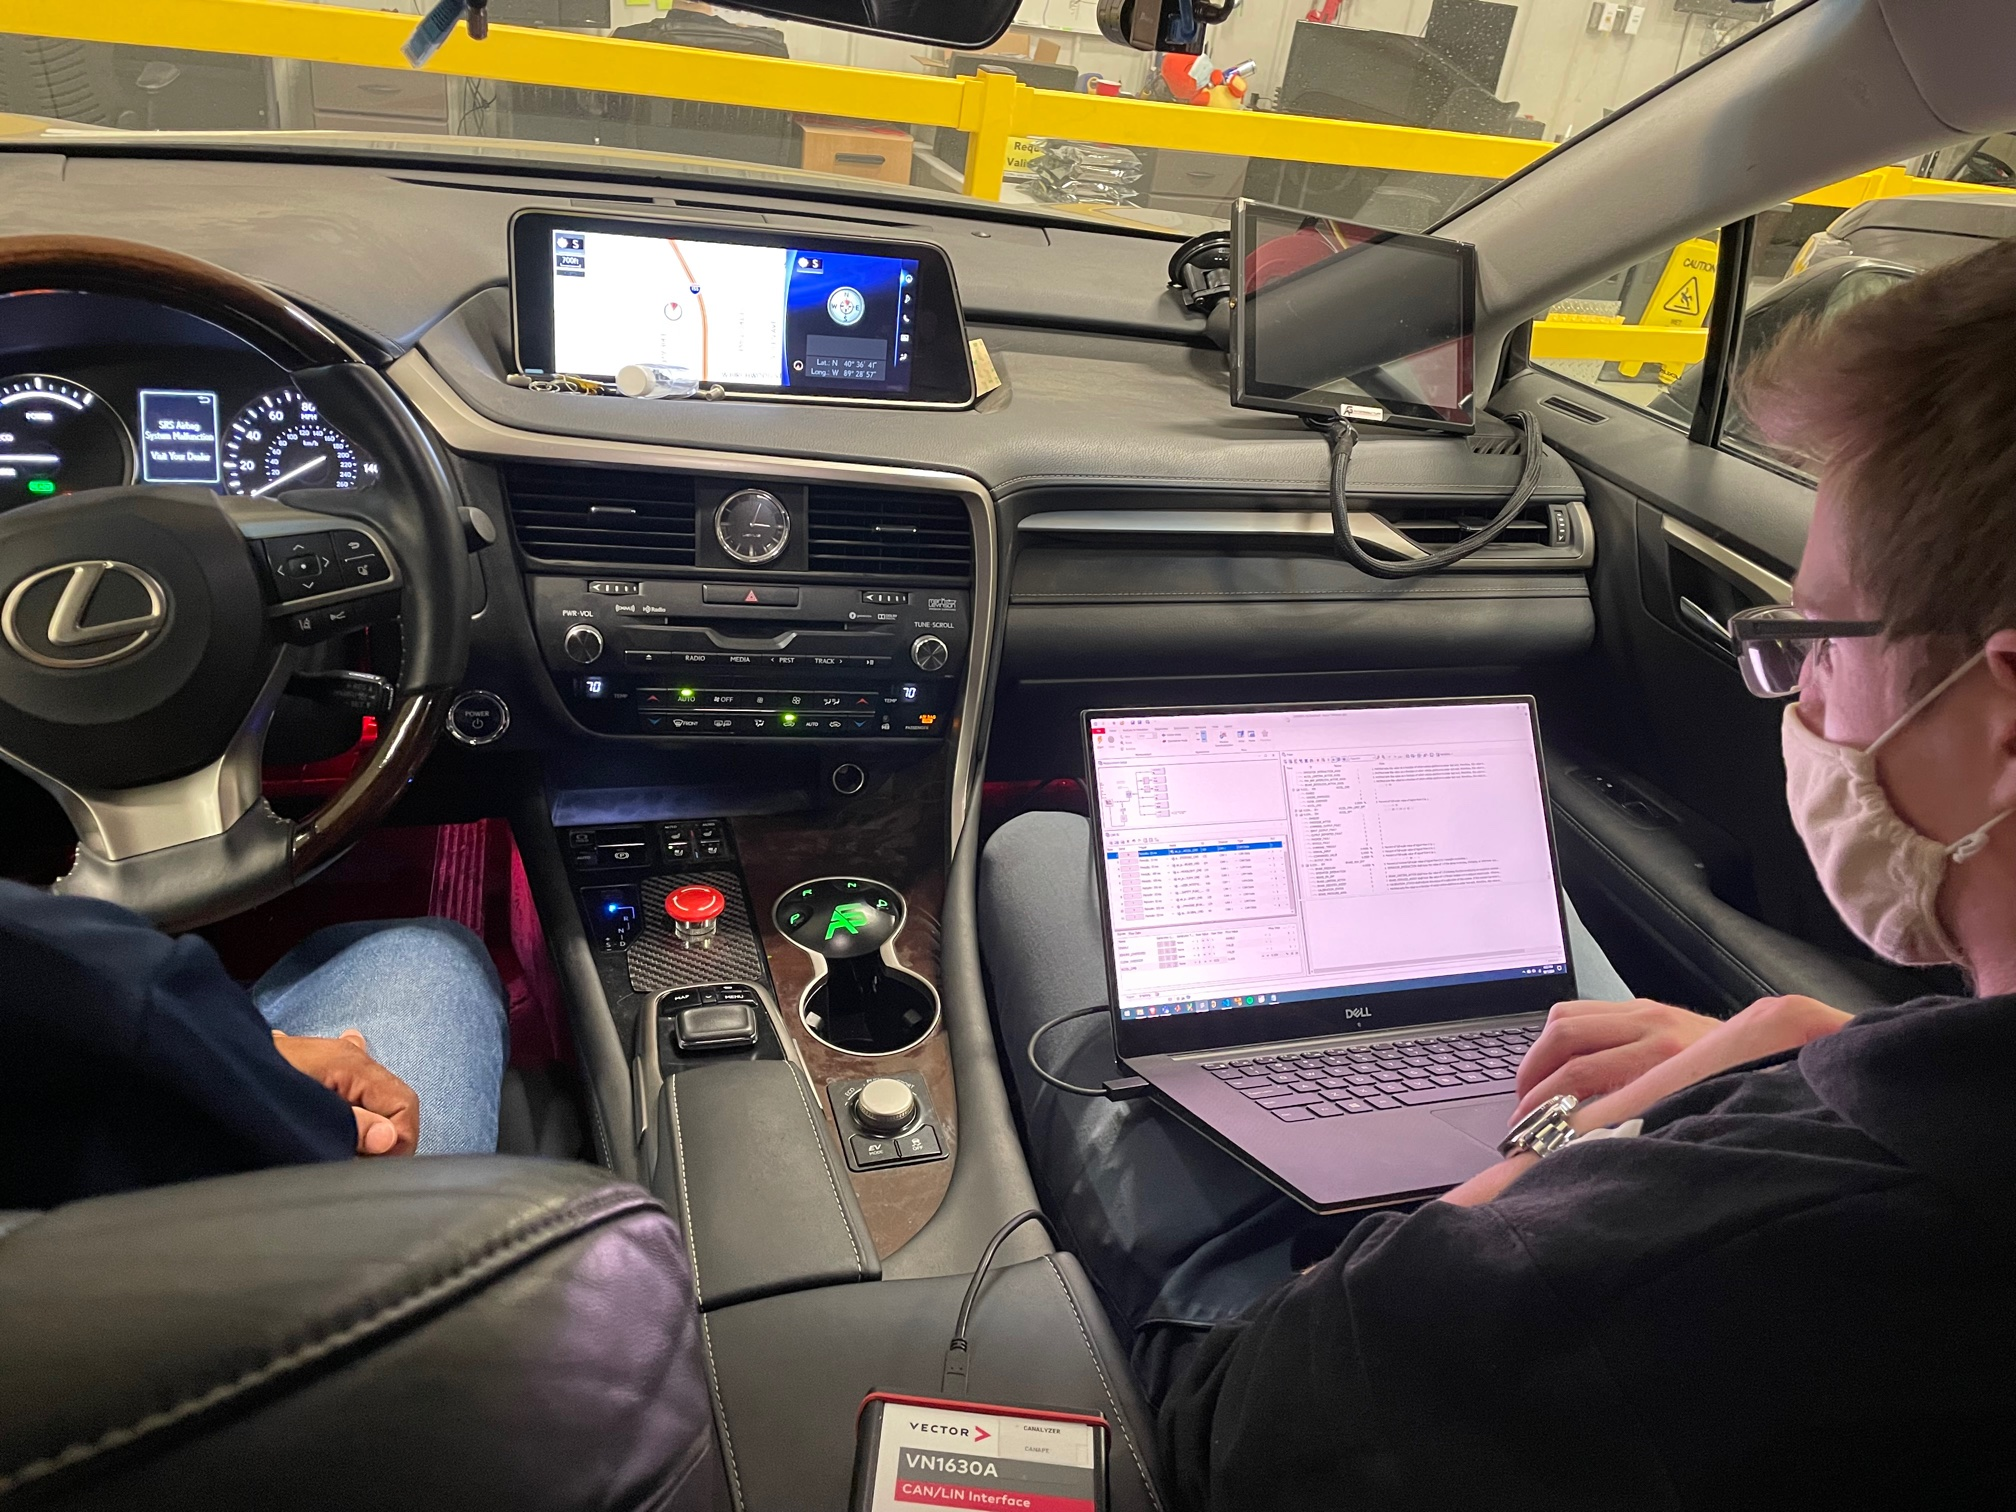
\includegraphics[width=.48\textwidth]{figs/img/picturesVisitToAStuff/dataColletionSetup1-20211007}
  \caption{Setup for collecting data in the Lexus RX450H self-driving vehicle.}
  \label{fig:vehicleSetup}
\end{figure}
%
The laptop is used to collect the data from the desired vehicle subsystem by the use of Vector's CANAlyzer software. The CAN Case collects data from the PAC Mod and ECU and sends the data using a CAN bus to the laptop which is then parsed and displayed through the use of CANAlyzer. The ECU and PAC Mod are not shown in Fig.~\ref{fig:vehicleSetup} as they are fixed behind panels of the vehicle. %

Using the data we collected for the steering, acceleration, and braking subsystems, we initially separated the data so we could analyze the by-wire and manual modes individually. This effort was made to identify if the models we developed could be used interchangeably regardless of what mode the autonomous vehicle subsystems were operating in. After analyzing the models we developed, we determined that they are not interchangeable as there were differences in the models. When the vehicle subsystem is in by-wire mode, the controller generates the torque voltages that are applied to each subsystem motor. As a result, we decided the most accurate model of each subsystem would be developed using the data when the subsystems are in manual mode. % For reference, the differences in the models created for by-wire and manual mode are depicted in Section \ref{subsec:SteeringTF} and \ref{subsec:AccelTF} for the steering and acceleration subsystems. For all other models we develop, we will only use manual mode data and will not create models for by-wire mode.


To develop the model of the steering, acceleration, and brake subsystems using a neural network architecture, we used one data subset to train the model and then used an additional subset of data to verify the model worked. The neural network model used a feedforward network that had one hidden layer containing three neurons. The model was also trained with twelve delay units to achieve the required accuracy, meaning that the first twelve output samples of the model should be ignored.
\subsection{Neural Network Modeling}
\label{sec:NN-Modeling}

\subsubsection{Steering System}
%
In Fig.~\ref{fig:InitialSteeringModel}, the top plot shows the simulated output of the neural network (Actual Output and Desired Output) when the input torque voltages and desired steering angle from a subset of data (subset~\#1) collected offline is fed into the model. The bottom plot shows the error between the desired steering angle and the output of the neural network. For the steering model, the error should be less than 5 degrees or approximately 0.1 radians. %Fig.~\ref{testedSteeringModel} shows the same plots except data subset 2 was used instead. %
%
\begin{figure}[htbp]
  \centering
  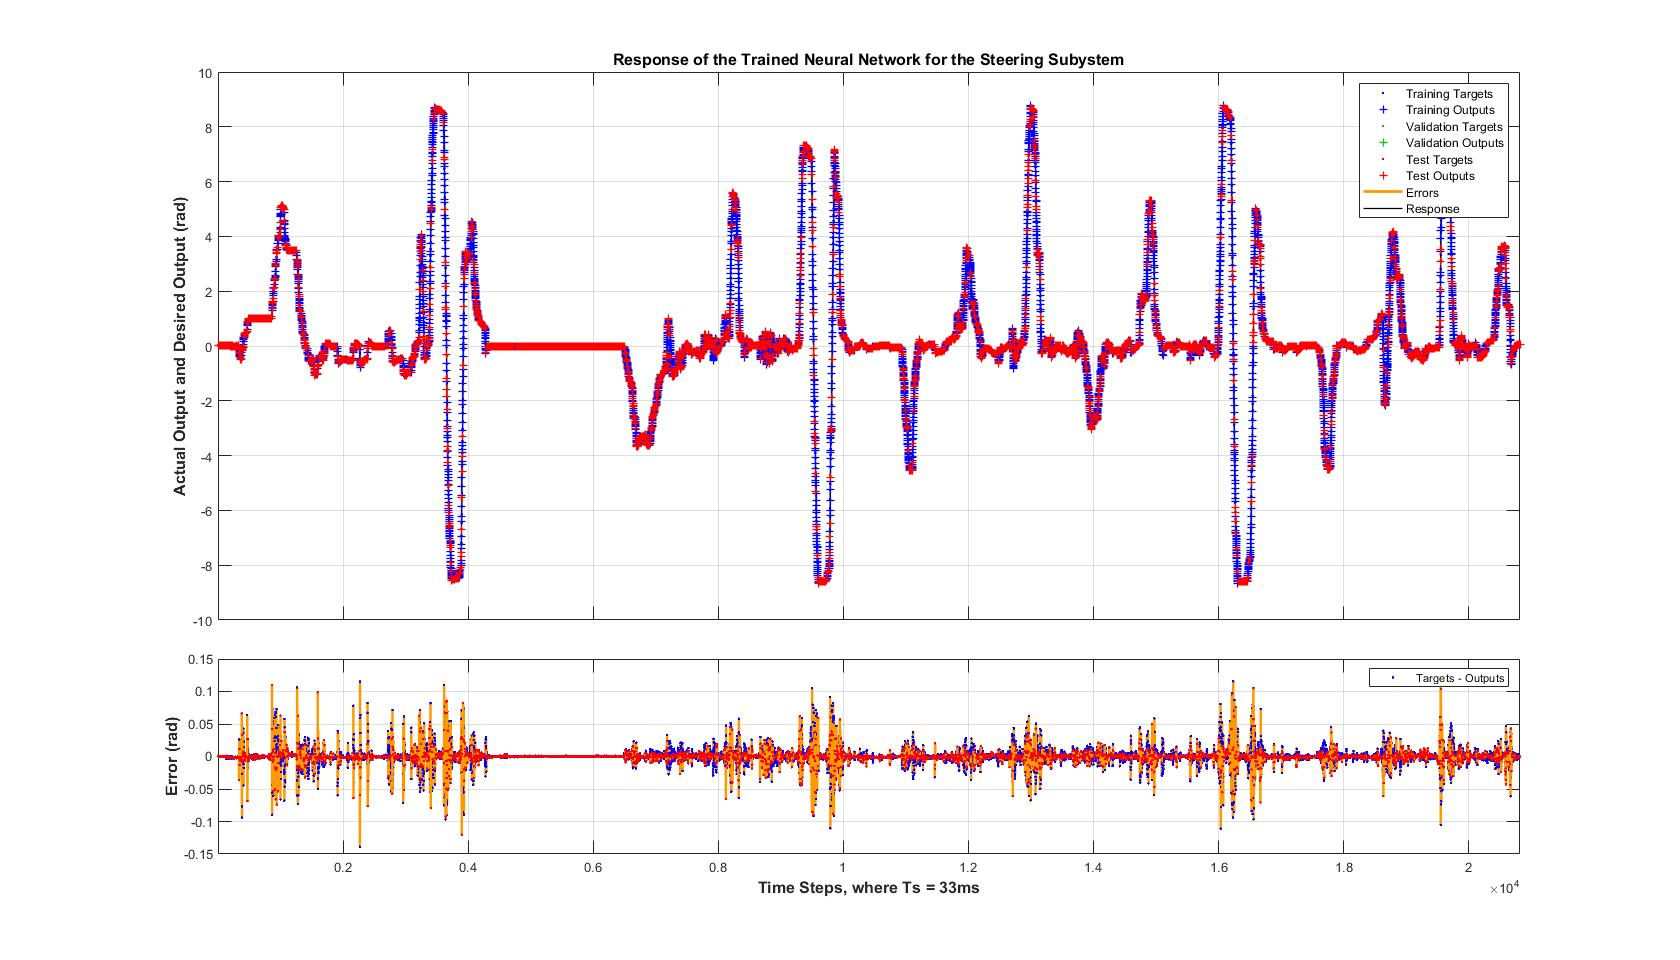
\includegraphics[width=0.90\linewidth]{figs/img/steeringNeuralNetworkTrainedOutput}
  \caption{Steering model performance in tracking desired steering angle and the error based on the data (subset 1).}
  \label{fig:InitialSteeringModel}
\end{figure}
%
% \begin{figure}[htbp]
% 	\centering
% 	\subcaptionbox{. \label{initalSteeringModel}}
% 		{}
% 	\subcaptionbox{Model Output Tracking and Error Plots for Data Subset 2 \label{testedSteeringModel}}
% 		{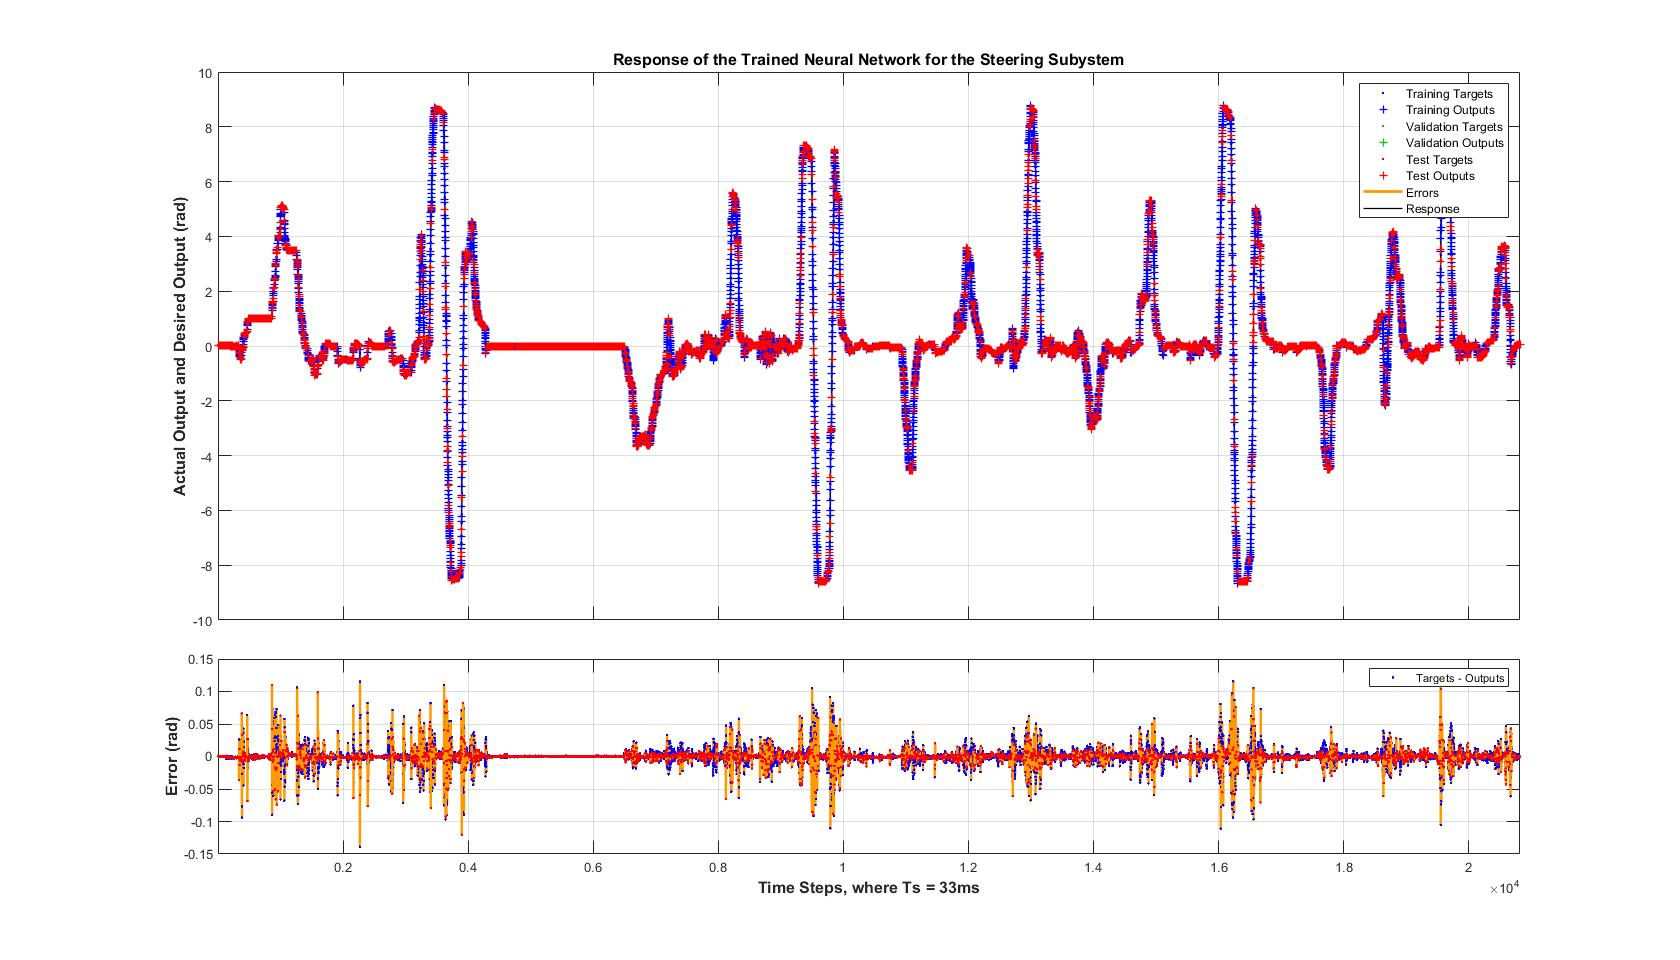
\includegraphics[width=0.90\linewidth]{figs/img/steeringNeuralNetworkTrainedOutput}}
% 	\caption{Steering System Training Plots}
% \end{figure}


\subsubsection{Acceleration System}
%
In Fig.~\ref{initalAccelModel}, the top plot shows the simulated output of the neural network when the input torque voltages and desired acceleration pedal position from data subset 1 are fed into the model. The bottom plot shows the error between the acceleration pedal position and the output of the neural network. For the acceleration model, the error should be less than 5\% or 0.05. Fig.~\ref{testedAccelModel} shows the same plots except data subset 2 was used instead. The model generated was able to follow the data from the logs very closely, and so met the accuracy requirements we had set. 

\begin{figure}[htbp]
	\centering
	\subcaptionbox{Model output tracking and Error Plots for Data Subset 1 \label{initalAccelModel}}
		{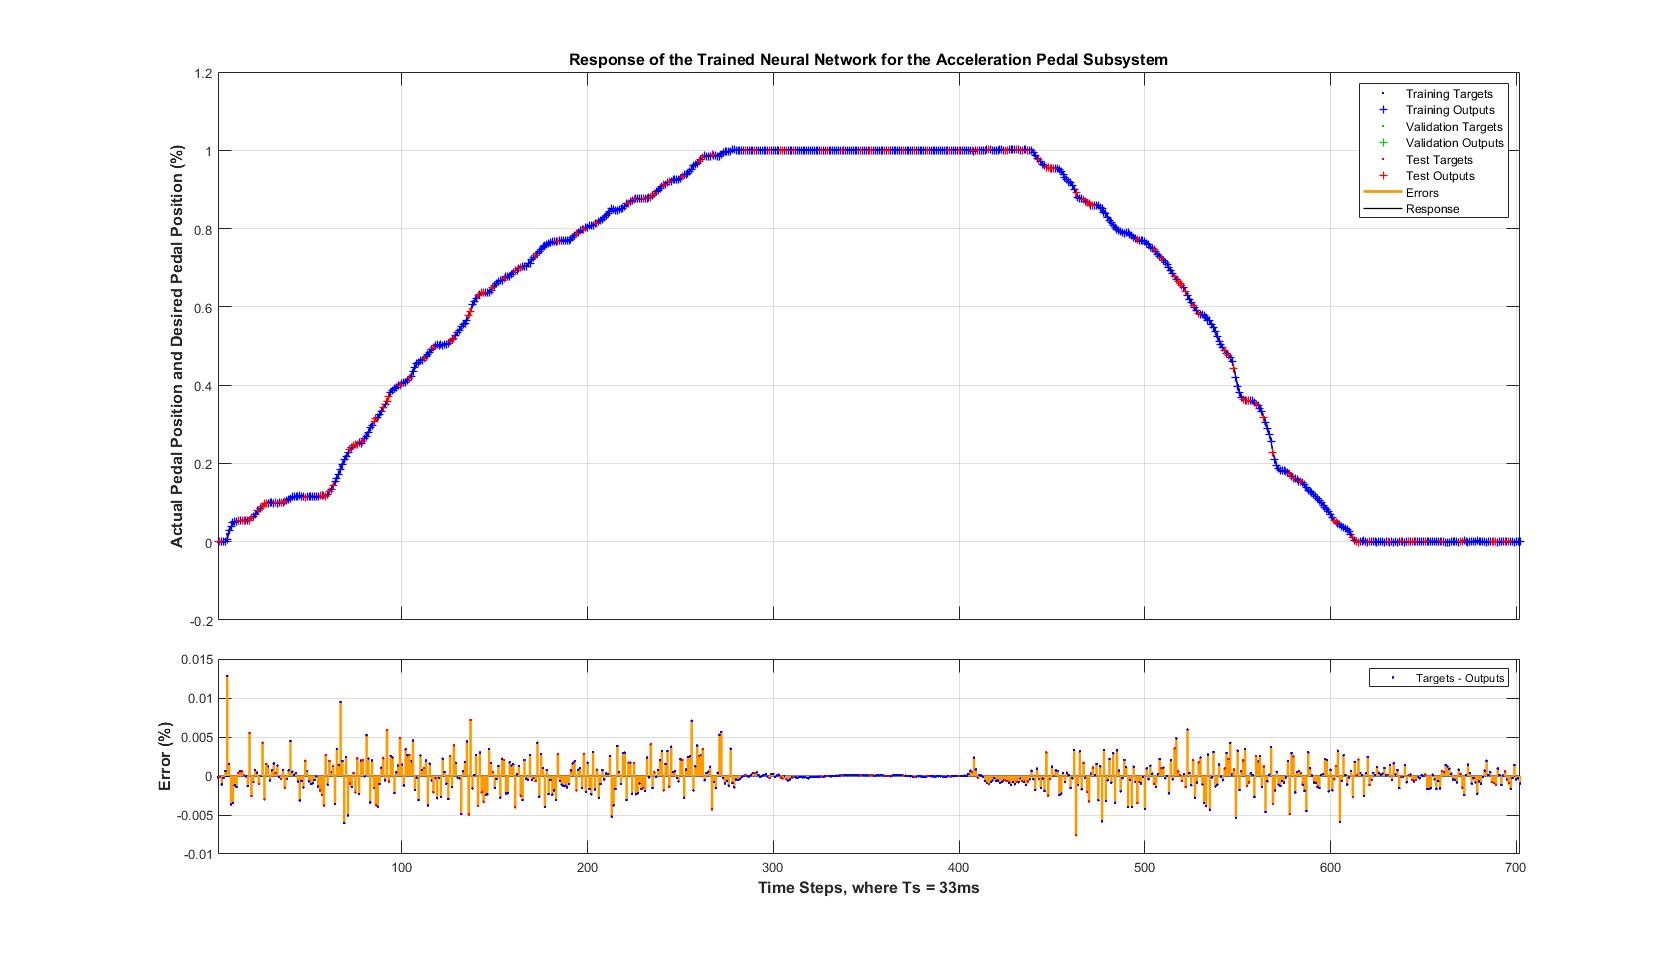
\includegraphics[width=0.90\linewidth]{figs/img/accelNeuralNetworkTrainedOutput}}
	\subcaptionbox{Model Output Tracking and Error Plots for Data Subset 2 \label{testedAccelModel}}
		{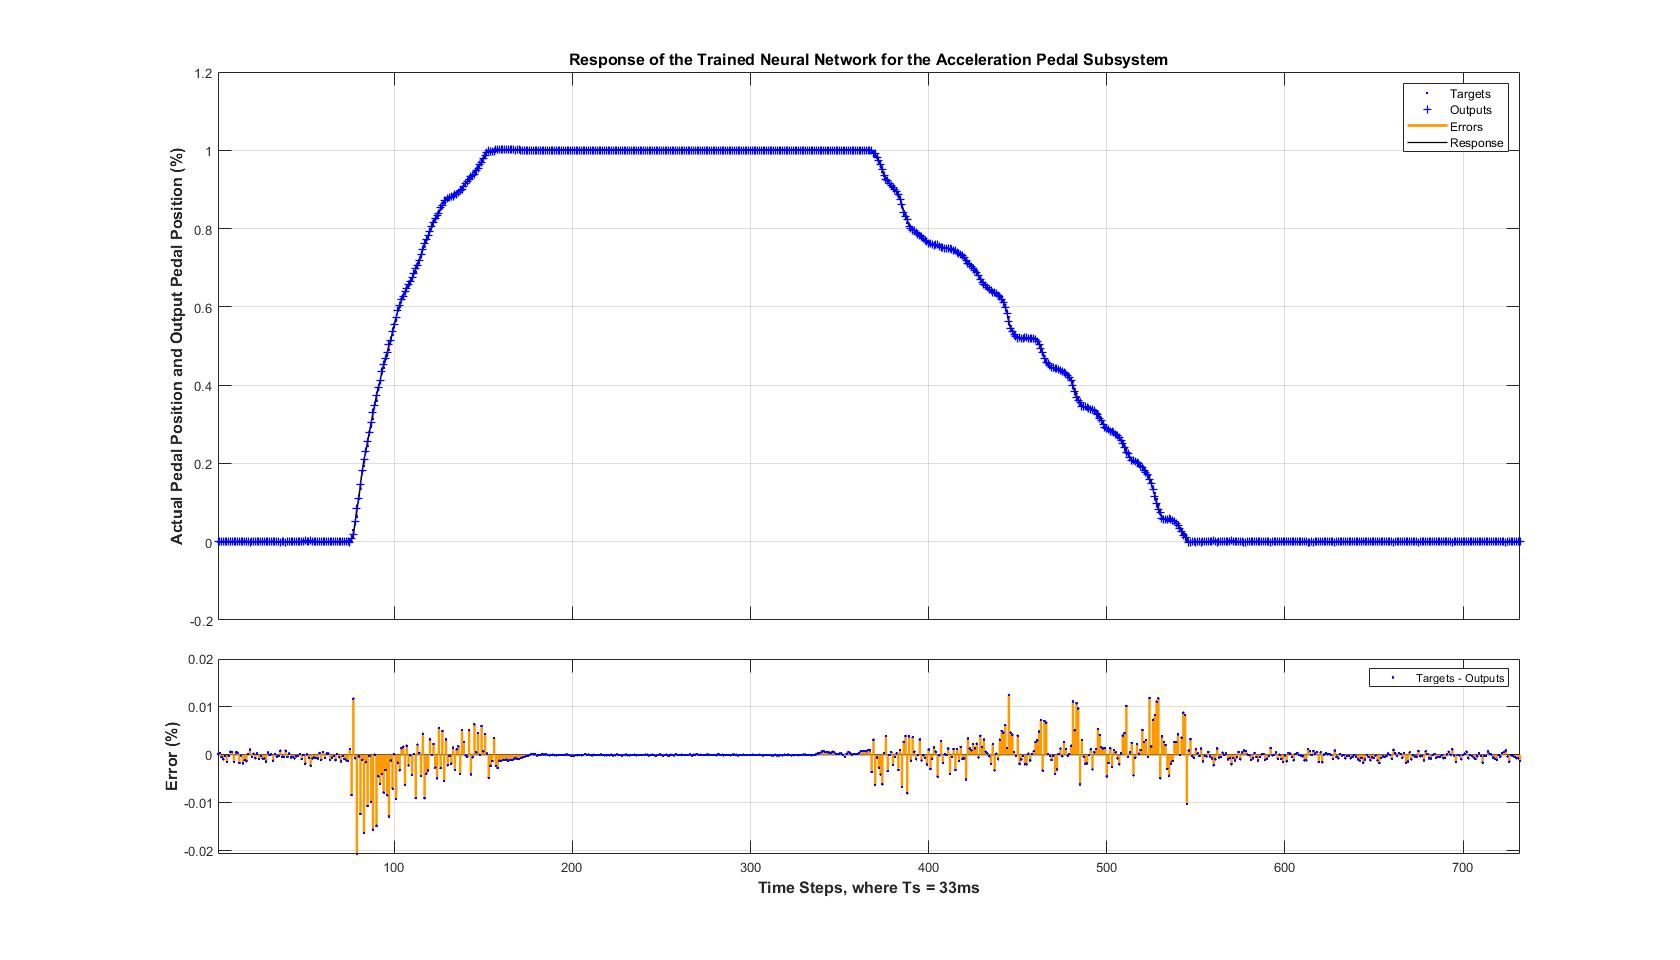
\includegraphics[width=0.90\linewidth]{figs/img/accelNeuralNetworkTrainedOutput2}}
	\caption{Acceleration System Training Plots}
\end{figure}


\subsubsection{Brake System}

The brake system was modeled using only the manual log data. It was trained using the data from the first brake log, and the result and error plots can be seen in Fig.~\ref{initalBrakeModel}. The plots show that the model is able to predict the outputs relatively accurately, along with keeping the error below 5\%. In order to further verify the accuracy of the model, it was tested using data from the second brake log. The results from that test, shown in Fig.~\ref{testedBrakeModel}, also show that the model can accurately predict the output values and do this within the accepted error bound of 5\%. The graphs show how the model tracks the data log and the error between the model output and the data log output. The y-axis for both graphs, “Output and Target” represents the Actual and Desired Brake Pedal Position as a percentage. Target represents the pedal position values from the brake data log we fed into our model. Output represents the pedal position values that the model produced. The x-axis for both graphs represents the Time Steps, with $T_s$ equal to 33ms. The brake subsystem neural network model was able to meet both the best fit and error requirements that had been set earlier, making it an accurate model. 

\begin{figure}[h]
	\centering
	\subcaptionbox{Model Output Tracking and Error Plots \label{initalBrakeModel}}
		{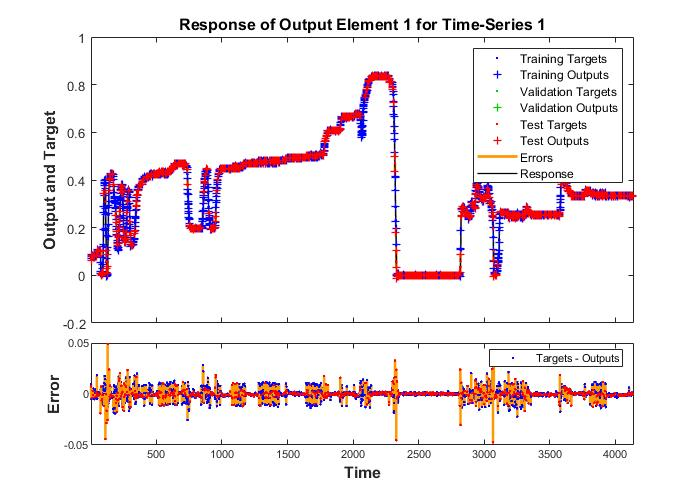
\includegraphics[width=0.90\linewidth]{figs/img/brake_new_neuralNetworkFig}}
	\subcaptionbox{Model Output Tracking and Error Plots for Log Two Data \label{testedBrakeModel}}
		{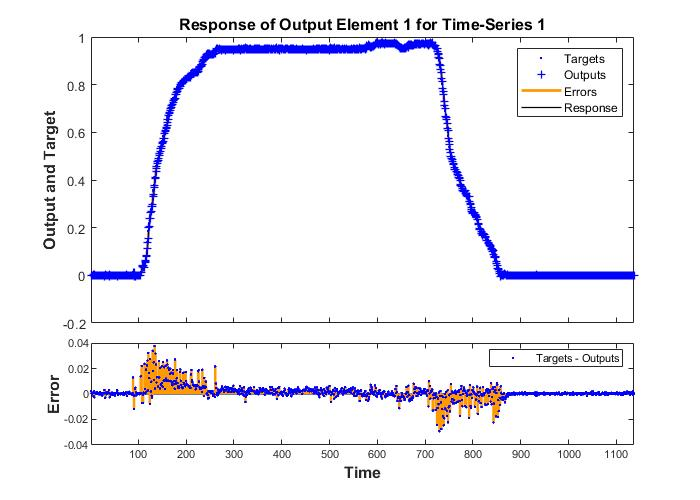
\includegraphics[width=0.90\linewidth]{figs/img/brake_new_neuralNetworkFigLog2Test}}
	\caption{Performance of the brake system modeling.}
\end{figure}



% The second test used constant blocks and To Workspace blocks to represent the voltages and desired pedal position in the first brake log. The results from this test also showed that the model was able to accurately track the data.


\subsection{Discussion}
\label{sec:discussion}

For each vehicle subsystem, the results show that the neural network models were the most accurate models. Other models that we developed, such as the transfer function models, were relatively accurate when tracking the data, but those models were consistently falling outside of the error bounds that were defined at the start of the project. The neural network models, however, track the data more accurately and reduced the error significantly so that all error requirements were met. We first proved that the neural network models that we developed were accurate using subsets of data as inputs to a Simulink model. Then we visited AutonomouStuff to generate the models on their HIL bench, as shown in Fig.~\ref{fig:hilBench}, using Control Desk to interface. Due to time constraints, AutonomouStuff was not able to get the proper hardware for this project connected to the HIL bench but we were able to test our models in an open-loop configuration and measure outputs to show that the correct voltages would be fed to any hardware that would be connected, shown in Fig.~\ref{fig:hilMeasuring}. One downside to using neural networks as the plant model is it causes some complexities when trying to include these models into the HIL bench software for use in developing and testing controllers.


\begin{figure}
    \centering
    \begin{subfigure}[b]{0.48\linewidth}
		\centering
    		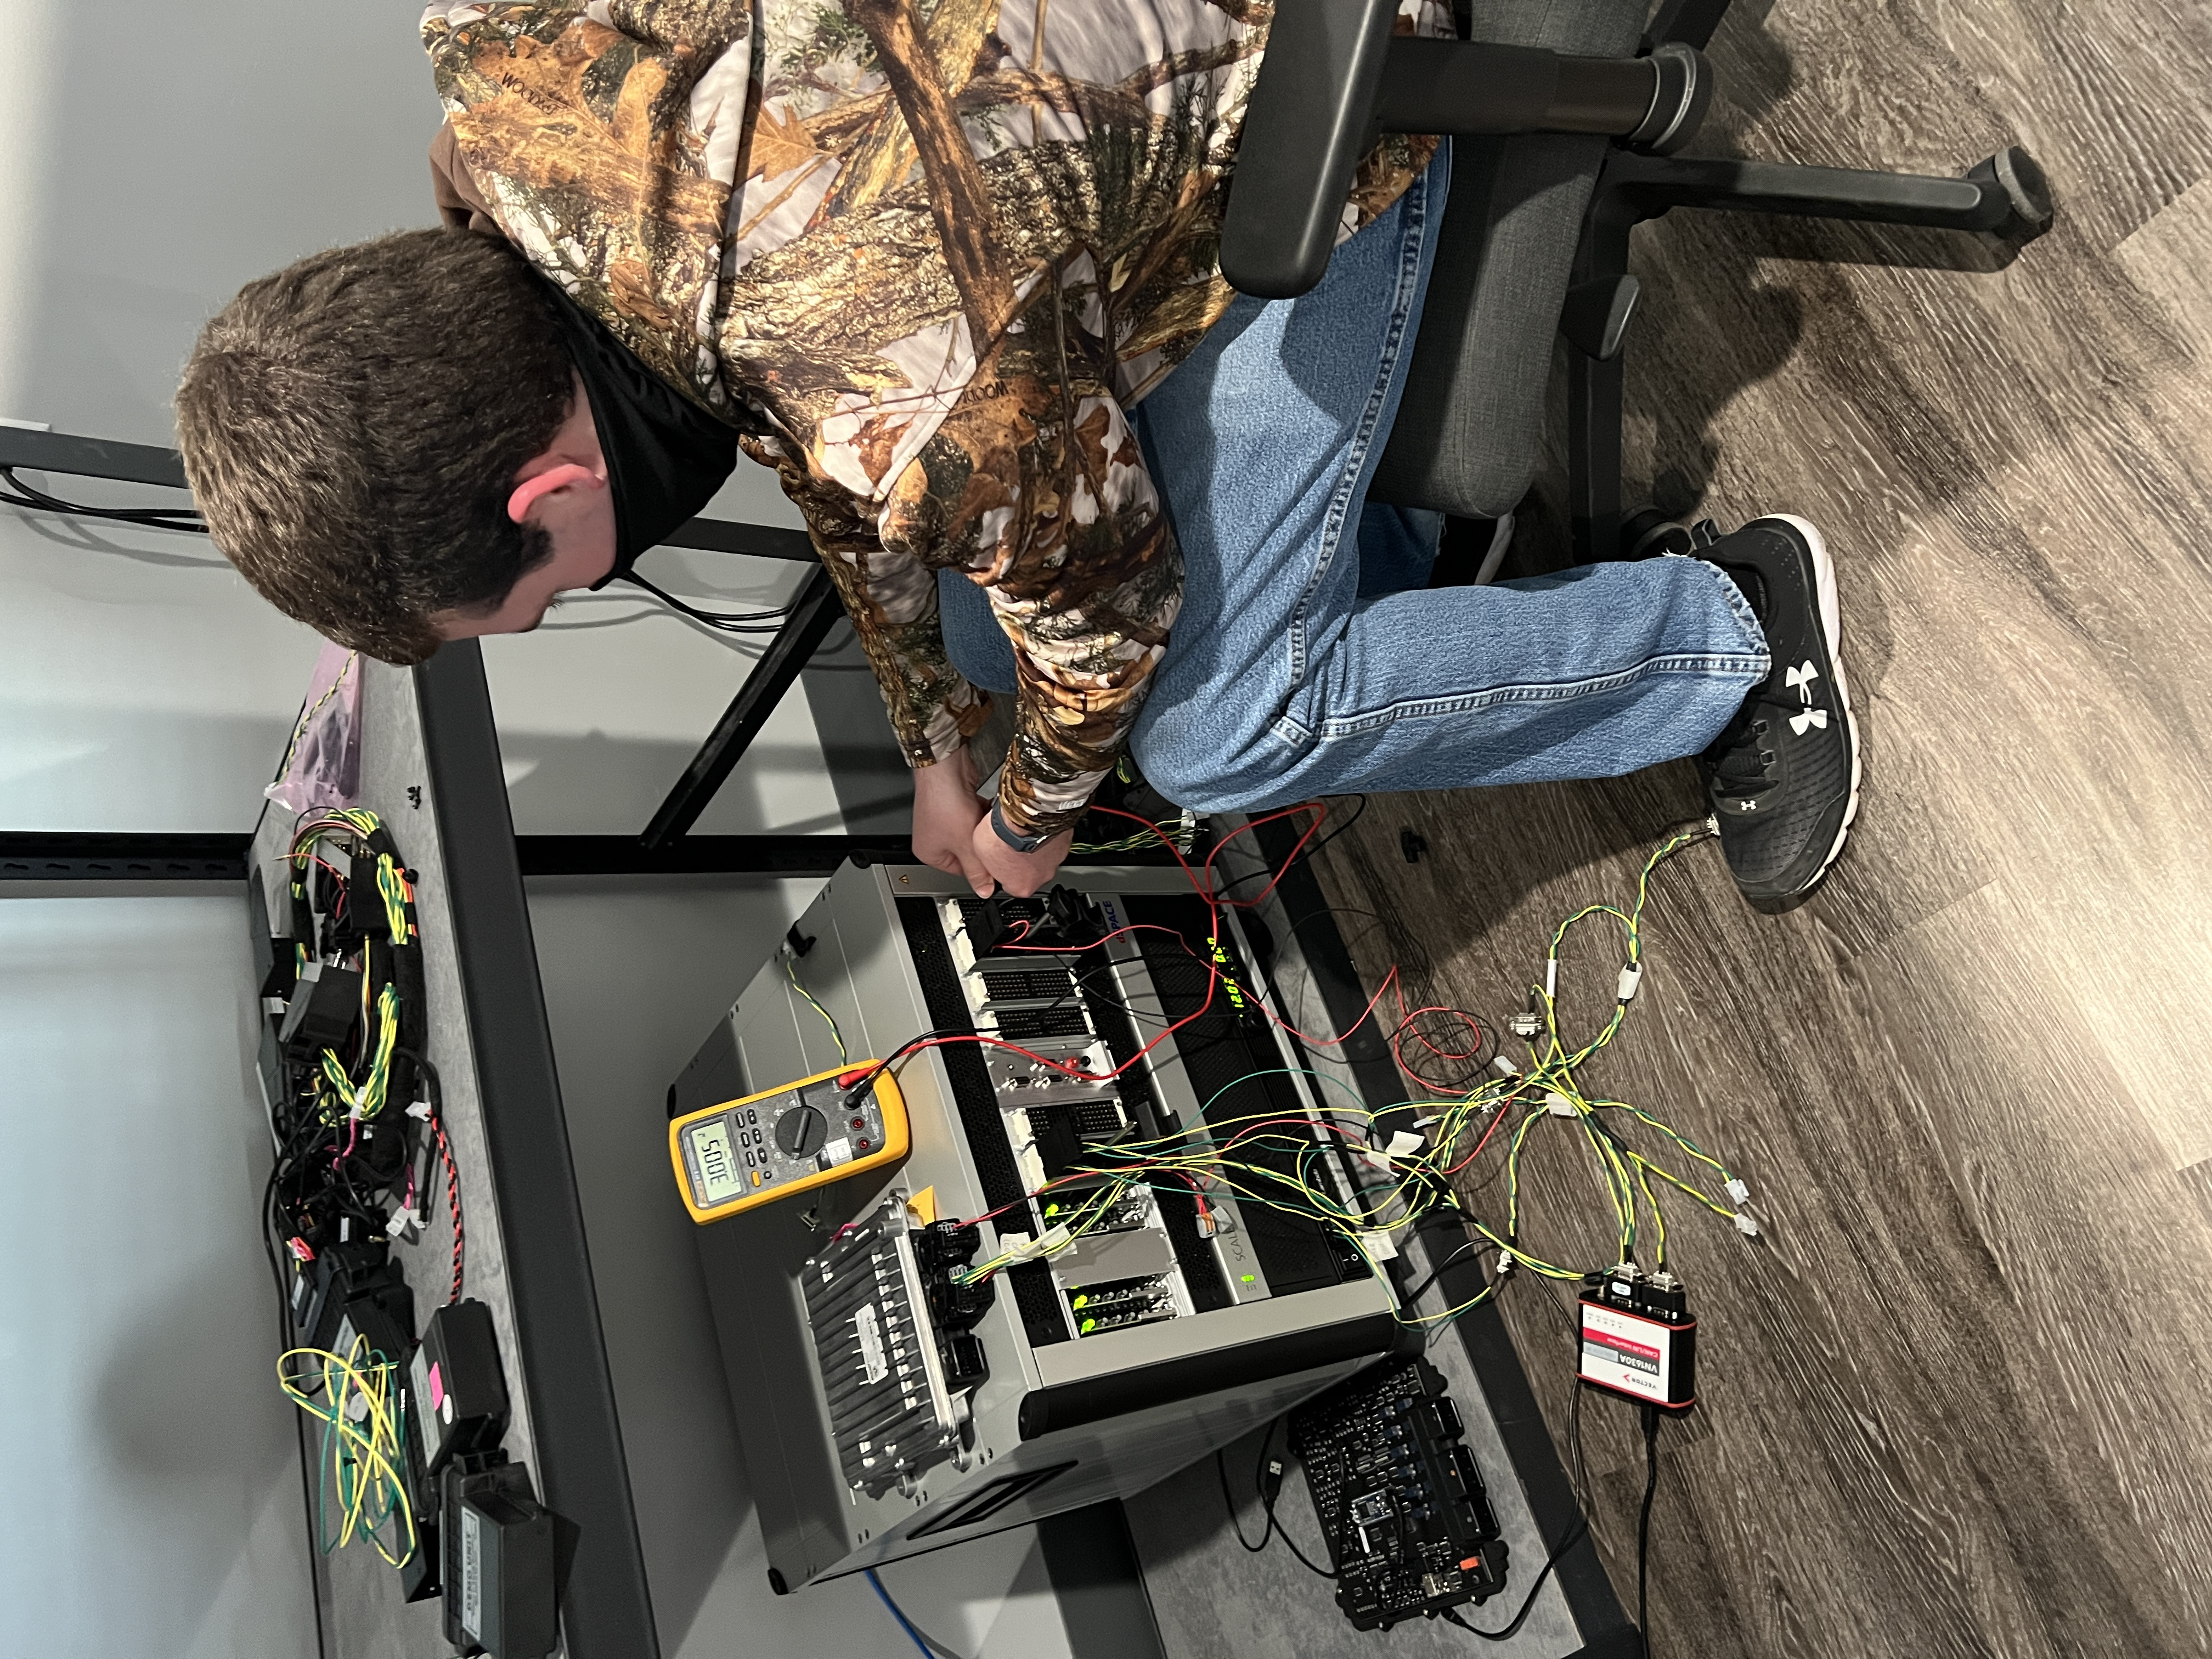
\includegraphics[angle=270,width=0.9\linewidth]{figs/img/picturesVisitToAStuff/aStuffVisit2Nick}
    		\caption{}
    \end{subfigure}
    \begin{subfigure}[b]{0.48\linewidth}
		\centering
    		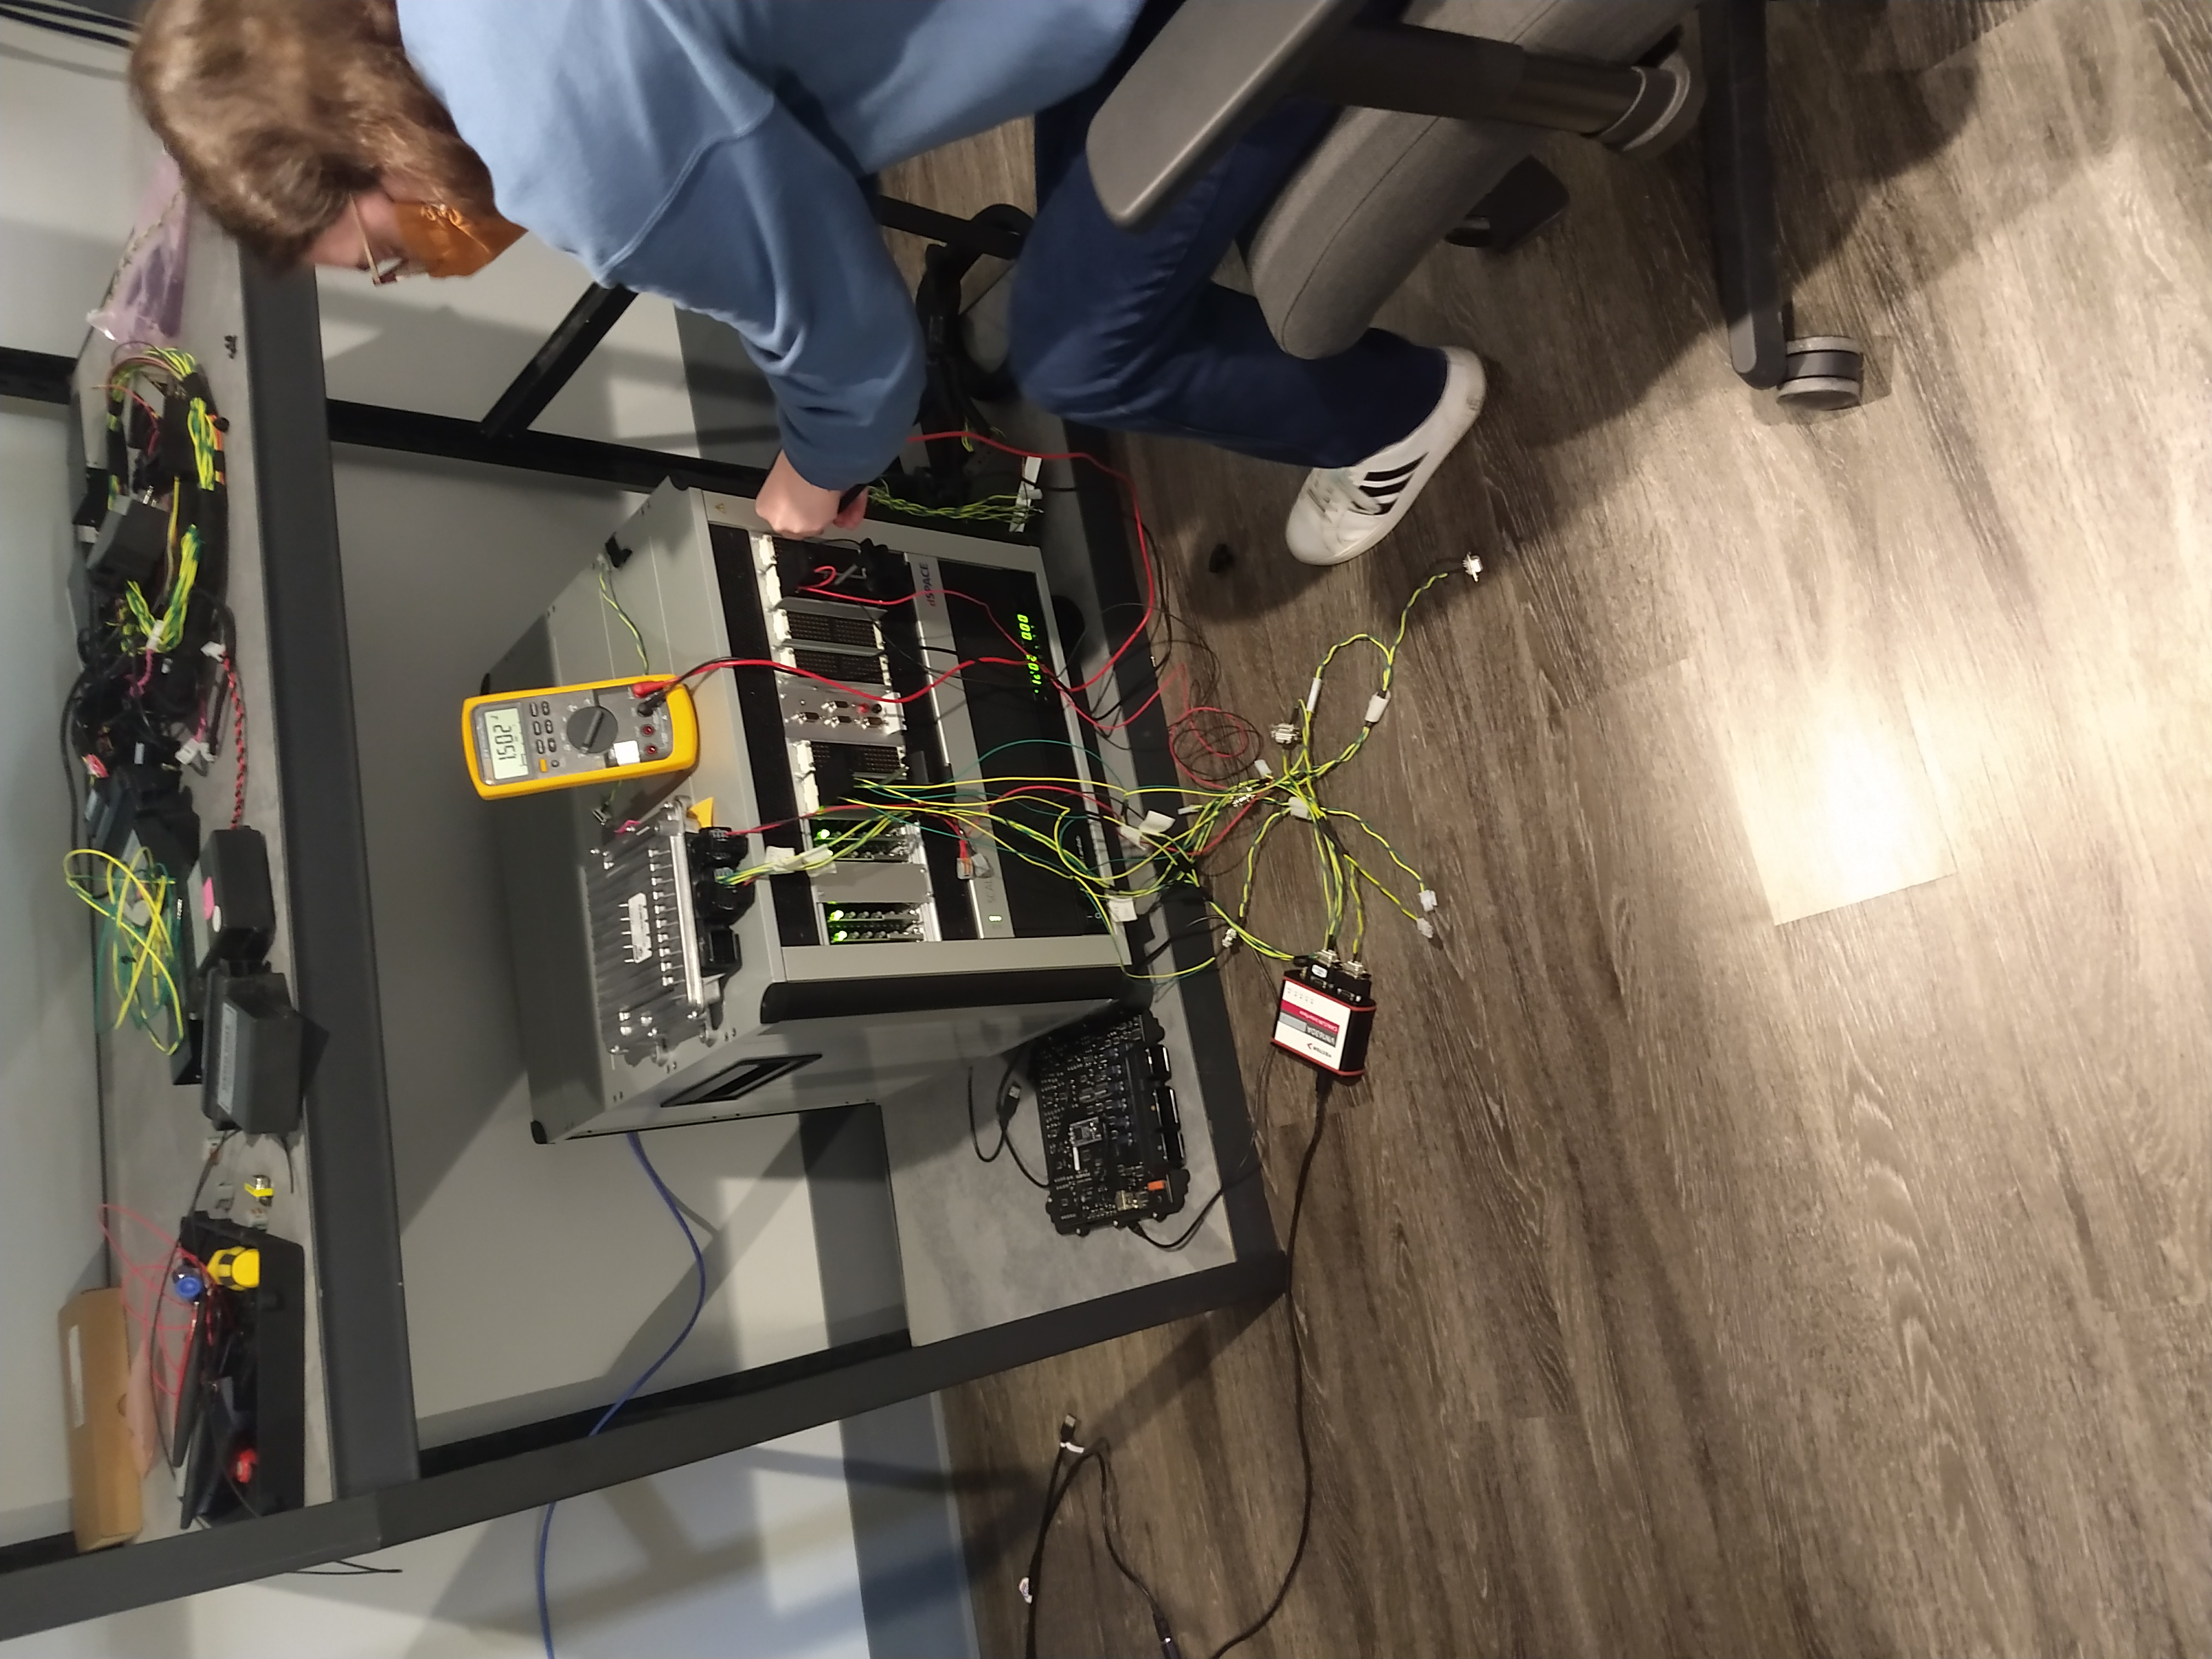
\includegraphics[angle=270,width=0.9\linewidth]{figs/img/picturesVisitToAStuff/hilMeasurementHannah}
    		\caption{}
    \end{subfigure}
    %\subfigure[b]{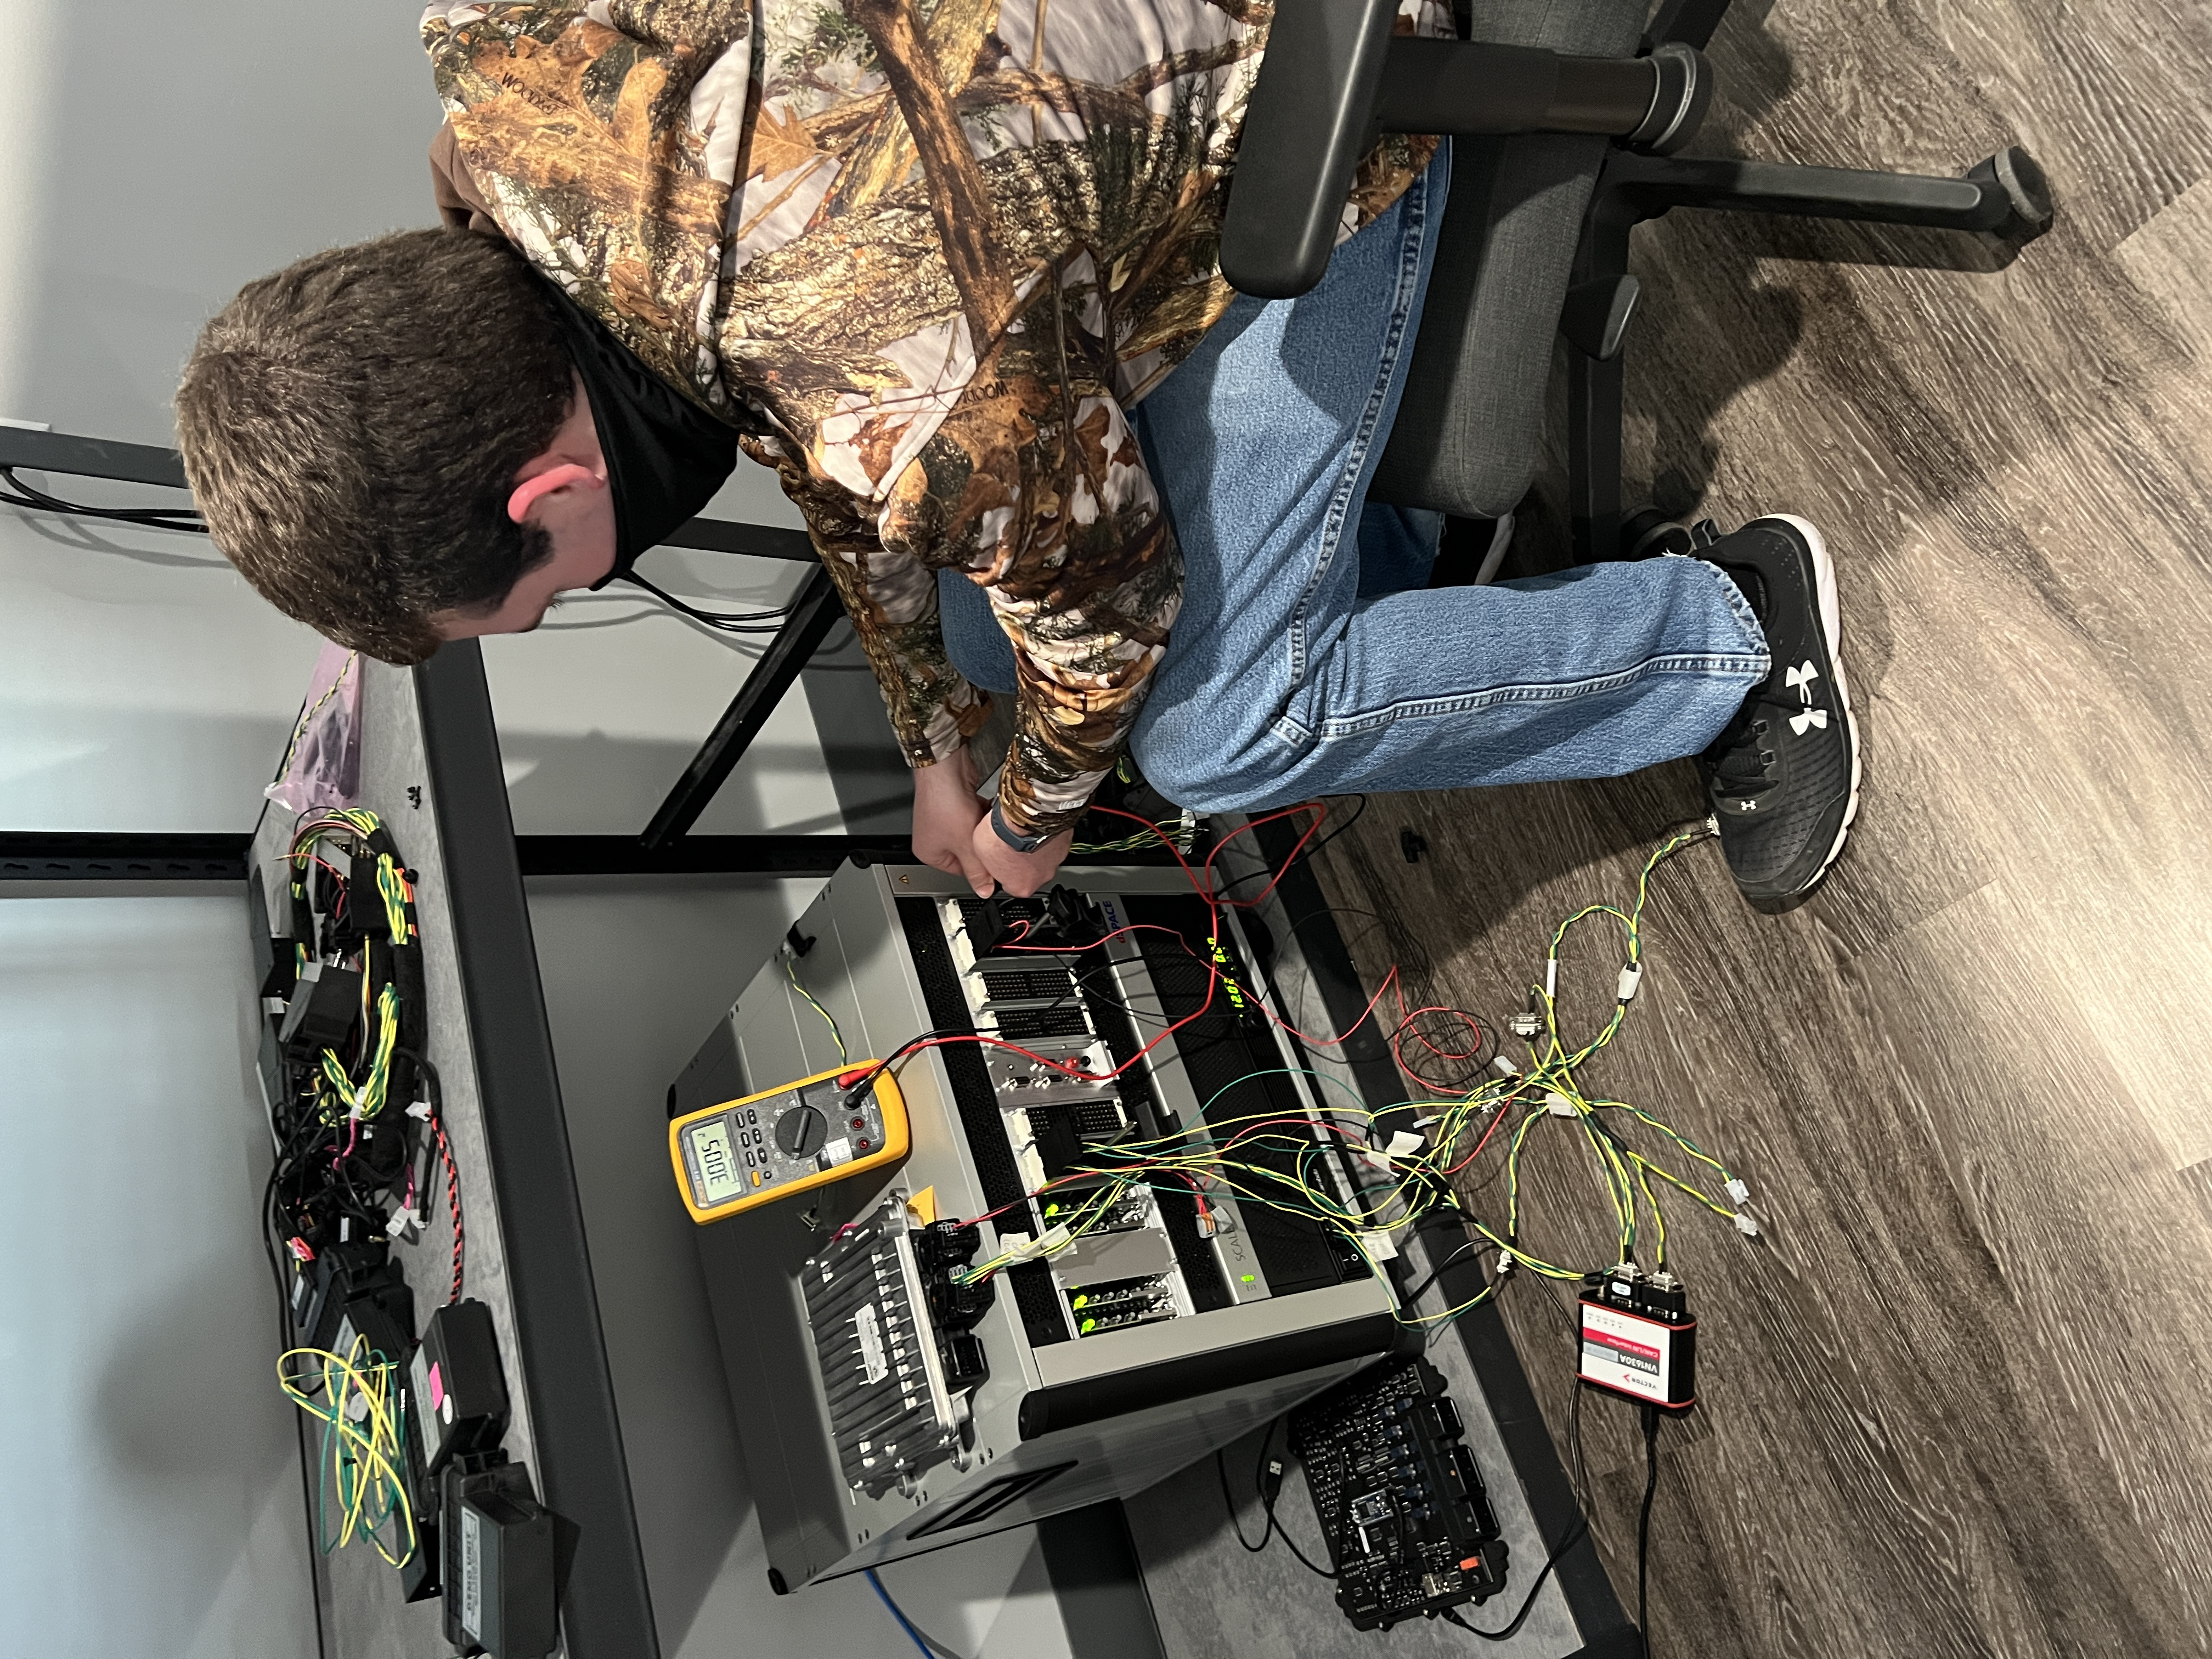
\includegraphics[width=0.48\linewidth]{figs/img/picturesVisitToAStuff/aStuffVisit2Nick}}
    %\subfigure[b]{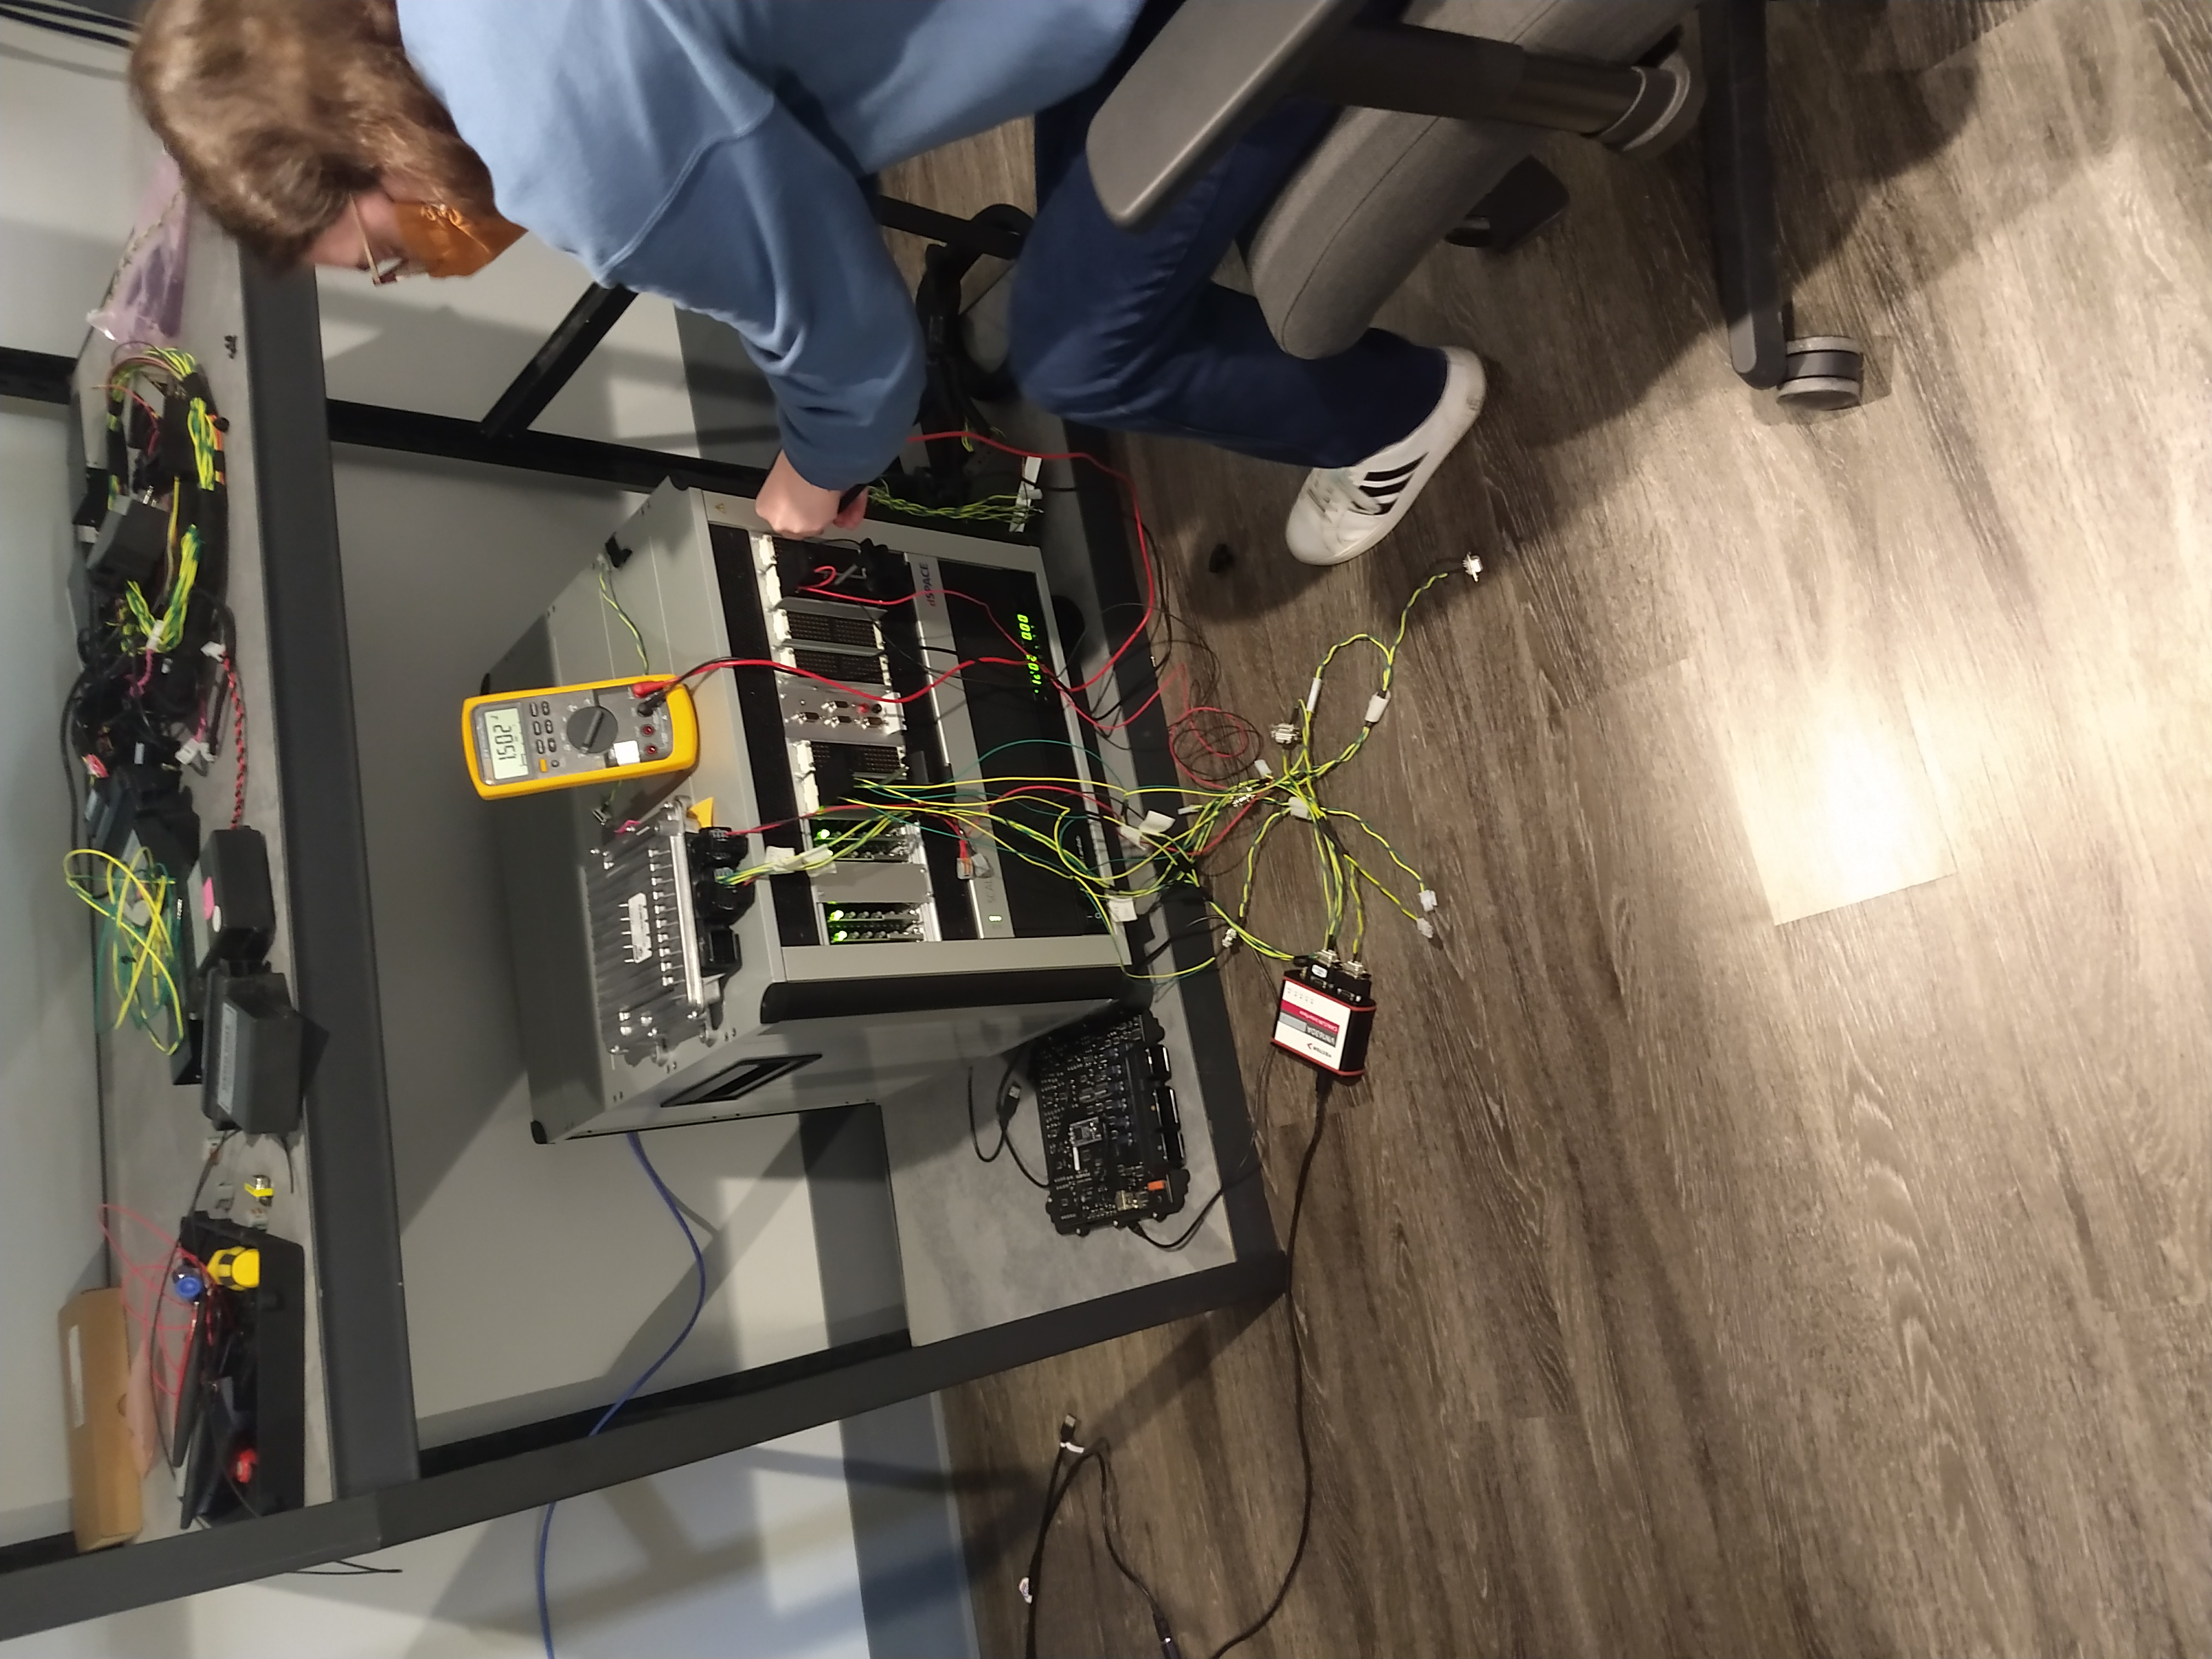
\includegraphics[width=0.48\linewidth]{figs/img/picturesVisitToAStuff/hilMeasurementHannah}}
    \caption{Verifying voltage measurements on the HIL bench.}
    \label{fig:hilMeasuring}
\end{figure}

\begin{figure}
  \centering
    \includegraphics[width=0.95\linewidth]{figs/inkscape/hilBenchAstuffAnnotatedNew}
  \caption{AutonomouStuff HIL bench configuration}
  \label{fig:hilBench}
\end{figure}

%\begin{figure}
%	\centering
%	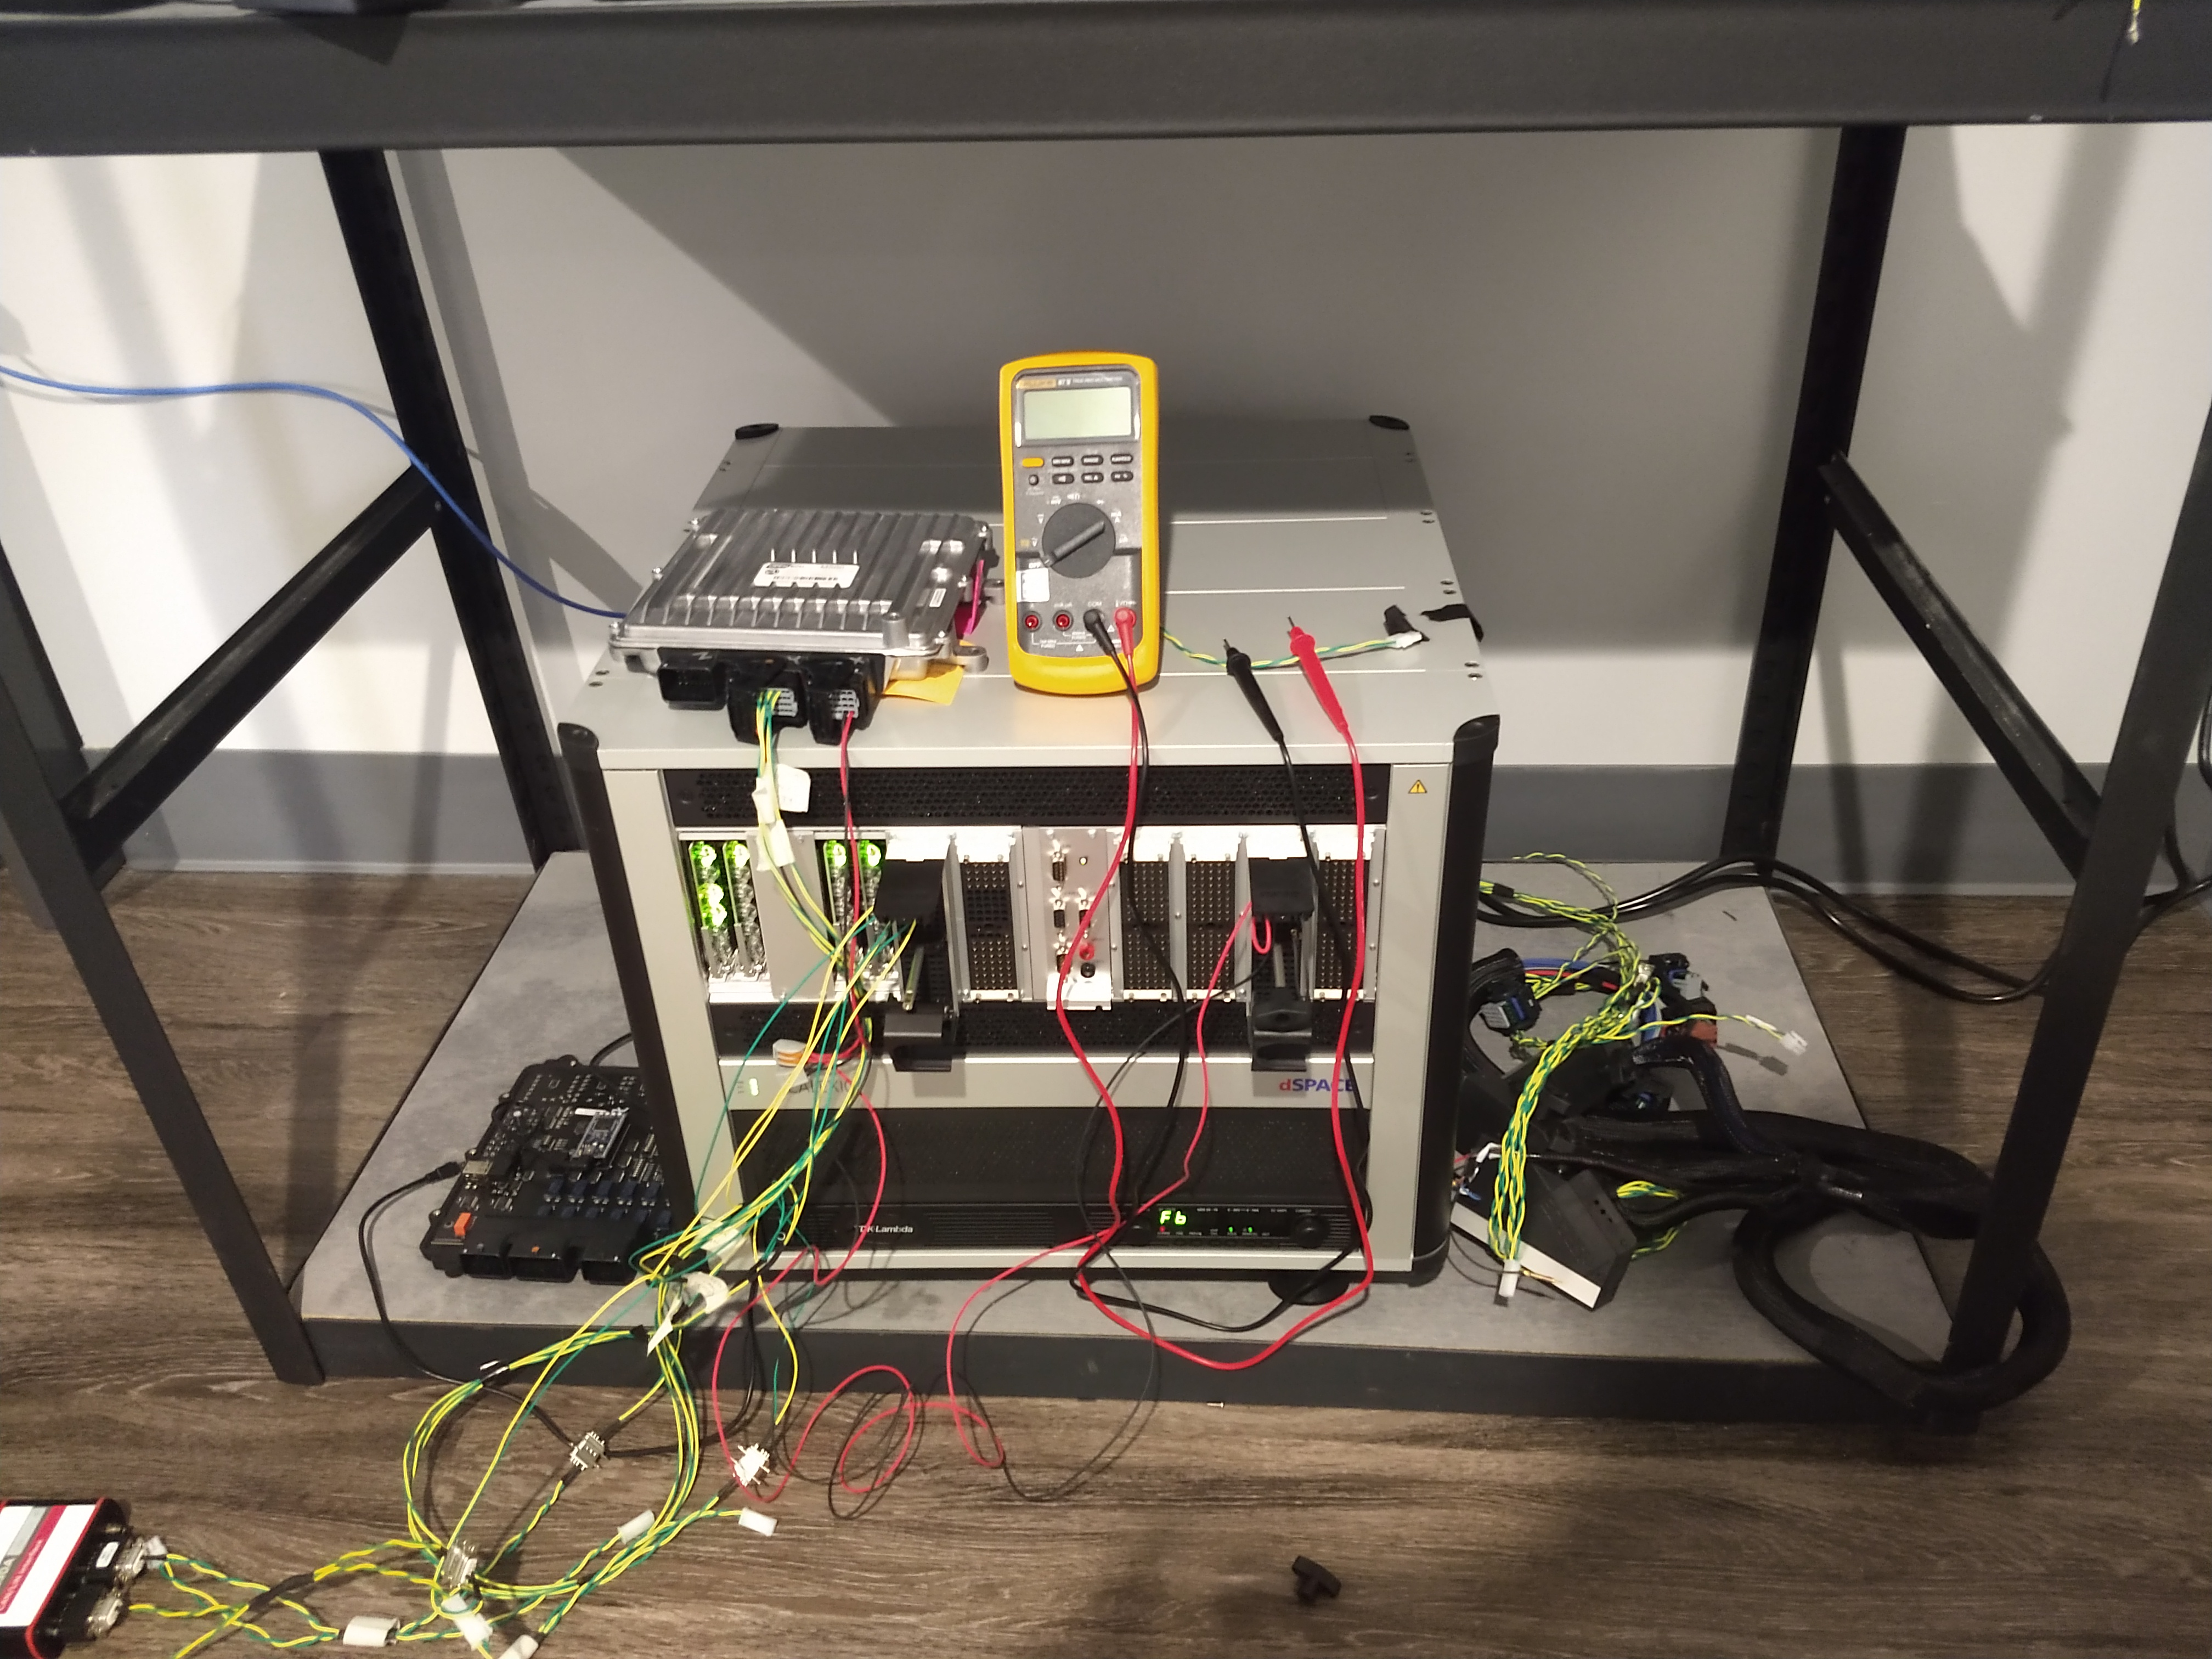
\includegraphics[width=0.95\linewidth]{figs/img/picturesVisitToAStuff/hilBenchAstuff}
%	\caption{AutonomouStuff HIL Bench Configuration}
%	\label{fig:hilBench}
%\end{figure}


\section{Conclusion and Future Work}
\label{sec:conclustionAndFutureWork}

In this paper, we presented the effectiveness of the data-driven hardware-in-the-loop plant modeling process using deep learning. The neural network time series modeling method  allowed us to train models using the data we collected. These models that were developed met the predefined accuracy requirements, and so were tested using an open loop setup. For conciseness, we presented HIL plant modeling for three subsystems, which are the steering, brake, and acceleration subsystems of the Lexus vehicle available at AutonomouStuff (the company who sponsored the project). Further testing should be completed for these subsystem models. Since time and availability constraints prevented us from testing the models using Hardware-in-the-Loop, further testing is important to make sure the developed models are accurate and compatible with testing using hardware. Future work  could be to start developing controllers based off of these models.

\clearpage
\bibliographystyle{IEEEtran}
\bibliography{bib/references.bib}

\end{document}
